%
% hps_thesis.tex
% author: Omar Moreno 
% date: August 31, 2015
%

% Set the document type and the font size
\documentclass[12pt]{ucthesis}

\usepackage[letterpaper, left=1.50in, right=1.25in]{geometry}

% Package from AMS that facilitates formula typography
\usepackage{amsmath}

% ?
\usepackage[utf8]{inputenc}

% Package required to load images
\usepackage{graphicx}

% Package used to add hyperlinks to references within a document
\usepackage{hyperref}

\usepackage{subcaption}

\usepackage{booktabs}

\usepackage{rotating}

% Package used to adjust the size of the section headings
\usepackage{titlesec}
\titleformat{\chapter}[display]
    {\LARGE\bfseries}{\chaptertitlename\ \thechapter}{20pt}{\LARGE}
\titleformat*{\section}{\large\bfseries}
\titleformat*{\subsection}{\normalsize\bfseries}

\def\dsp{\def\baselinestretch{1.8}\large\normalsize}
\dsp

\begin{document}

%%%%%%%%%%%%%%%%
% Front Matter %
%%%%%%%%%%%%%%%%

\title{Search for a Heavy Photon in the 2015 Heavy Photon Search Engineering Run Data}
\author{Omar Moreno}
\degreeyear{2016}
\degreemonth{June}
\degree{DOCTOR OF PHILOSOPHY}
\numberofmembers{3}
\chair{Professor Bruce Schumm}
\committeememberone{Professor Jason Nielson}
\committeemembertwo{Professor Abe Seiden}
\field{PHYSICS}
\campus{Santa Cruz}
\deanlineone{Tyrus Miller}
\deanlinetwo{Vice Provost and Dean of Graduate Studies}
\deanlinethree{}

\begin{frontmatter}

    \maketitle
    \copyrightpage
    
    \tableofcontents
    \listoffigures
    \listoftables

    %%%%%%%%%%%%%%%%
    %   Abstract   %
    %%%%%%%%%%%%%%%%
    \begin{abstract}
        
\pagestyle{plain}
The Heavy Photon Search (HPS) is a new experiment at Jefferson Lab that will 
search for heavy $U(1)$ vector bosons (heavy photons, dark photons or $A'$)
in the mass range of 10 MeV/c$^{2}$ to 1 GeV/c$^{2}$ that couple weakly to
ordinary matter.  Heavy photons in this mass range are theoretically favorable
and may also mediate dark matter interactions.  The heavy photon couples to 
electric charge through kinetic mixing with the photon, in turn, inducing an 
effective gauge coupling of the $A'$ to electric charge, which is suppressed
relative to the electron charge by a factor of 
$\epsilon \sim 10^{-2} - 10^{-12}$.  Since heavy photons couple to electrons, 
they can be produced through a process analogous to bremsstrahlung radiation, 
subsequently decaying to narrow $e^{+}e^{-}$ resonances which can be observed 
above the dominant QED trident background.  For suitably small couplings, dark
photons travel detectable distances before decaying, providing a second 
signature.

HPS will utilize this production mechanism to probe heavy photons with relative 
couplings of $\epsilon^2 \sim 10^{-5} - 10^{-10}$ and search for the 
$e^{+}e^{-}$ decay of the
heavy photon via two signatures: invariant mass and displaced vertex.  Using 
Jefferson Lab’s high luminosity electron beam incident on a thin tungsten target along with a compact, large 
acceptance forward spectrometer consisting of a silicon vertex tracker and lead
tungstate electromagnetic calorimeter, HPS will access unexplored regions in the
mass-coupling phase space. 

The HPS engineering run took place in spring of 2015 using a 1.056 GeV, 50 nA 
beam.  This dissertation will present the results of a resonance search for a heavy
photon in the mass range between 20 MeV/$c^2$ to 60 MeV/$c^2$ using a portion of the unblinded
engineering run data which amounts to a luminosity of 74 nb$^{-1}$
(.4671 mC of charge).

    \end{abstract}

    \begin{dedication}
        \null\vfil
        {
            \large
            \begin{center}
                To me, myself and I.
            \end{center}
        }
        \vfil\null
    \end{dedication}

    \begin{acknowledgements}
    \end{acknowledgements}

\end{frontmatter}

%%%%%%%%%%%%%%%%%%%%
%   Introduction   %
%%%%%%%%%%%%%%%%%%%%

\chapter{Motivations}

The existence of additional $U(1)$ gauge symmetries of nature are common in
several Beyond the Standard Model (BSM) theories 
\cite{Goodsell:2010ie, Abel:2008ai, Candelas:1985en, Andreas:2011in, Jaeckel:2010ni}.
Such theories envision the associated gauge boson  inhabiting a  ``hidden sector'' consisting of a complex of 
particles and gauge bosons.  Probing the structure of such a hidden sector may
be possible through the so called ``Vector'' portal which describes  
the weak coupling of the $A'$ to charged particles through ``kinetic mixing''
with the photon. In fact, it is natural for the $A'$ to 
kinetically mix with the Standard Model (SM) photon through the interaction
of massive fields carrying both SM hypercharge and dark charge \cite{Holdom:1985ag}.
The mixing of the photon with the $A'$ would not only allow searching for
new hidden sector particles, but also dark matter which some theoretical models
have envisioned as inhabiting the hidden sector, with it's interactions mediated
via an $A'$ \cite{ArkaniHamed:2008qn, Pospelov:2008jd, cheung2009, ArkaniHamed:2008qp}.

The chapter that follows will motivate the need to search for an $A'$.  
This will include an overview of current astrophysical anomalies
that may be explained assuming a dark matter candidate that couples to a 
heavy photon.  Finally, a review of current experimental limits on the $A'$ 
coupling strength will be given.

\section{Theoretical Formalism and Physics Motivation}

As Holdom \cite{Holdom:1985ag} realized in the mid eighties, in a theory with 
$U(1)_Y \times U(1)'$, there is a term in the gauge part of the Lagrangian 
that allows $U(1)_Y$ and $U(1)'$ to mix.  The gauge part of such a theory can
be written as
\begin{equation}
    \mathcal{L}_{\text{gauge}} = - \frac{1}{4} F_Y^{\mu \nu}F_{Y, \mu \nu}
                          - \frac{1}{4} F'^{\mu \nu}F'_{\mu \nu}
                          + \frac{1}{2} \epsilon F'^{\mu \nu} F_{Y, \mu \nu}
    \label{eqn:l_gauge}
\end{equation}
%the associated gauge boson (heavy photon,
%dark photon or $A'$) can couple to the SM photon through the ``kinetic mixing''
%interaction
where $F'_{\mu \nu} = \partial_{\mu}A'_{\nu} - \partial_{\nu}A'_{\mu}$ 
($F^{\mu \nu}_{Y} = \partial^{\mu}A^{\nu} - \partial^{\nu}A^{\mu}$) is the
field strength tensor of the heavy photon (SM hypercharge) and $\epsilon$ is a
dimensionless coupling constant.  Illuminating the low-energy effects that result
from kinetic mixing can be achieved by decoupling the gauge fields through the
redefinition of the SM hypercharge gauge field as
\begin{equation}
    A_{\mu} \rightarrow A_{\mu} + \epsilon A'_{\mu}.
\end{equation}
Ignoring all $\epsilon^2$ terms that arise from such a transformation, this
results in the diagnolization of \ref{eqn:l_gauge} as
\begin{equation}
    \mathcal{L}_{\text{gauge}} = - \frac{1}{4} F_Y^{\mu \nu}F_{Y, \mu \nu}
                          - \frac{1}{4} F'^{\mu \nu}F'_{\mu \nu}.
\end{equation}
However, the redefinition of the field also affects the interaction term of 
the Lagrangian, $\mathcal{L}_{int} = A^{\mu}J_{\mu}^{EM}$ as
\begin{equation}
    A^{\mu}J_{\mu}^{EM} \rightarrow (A^{\mu} + \epsilon A'^{\mu})J_{\mu}^{EM}.
\end{equation}
As a result, an effective coupling is induced between the electromagnetic current and 
the heavy photon field that is suppressed by a factor of $\epsilon$.

If $U(1)_Y$ is embedded in a Grand Unified Theory, kinetic mixing between the
SM photon and the heavy photon can naturally be generated at loop-level 
assuming there exists heavy multiplets, ($\Phi$, $\Phi'$), 
that are charged under both the SM hypercharge and dark charge 
(see Fig. \ref{fig:ap_loop}).
\begin{figure}
    \centering
    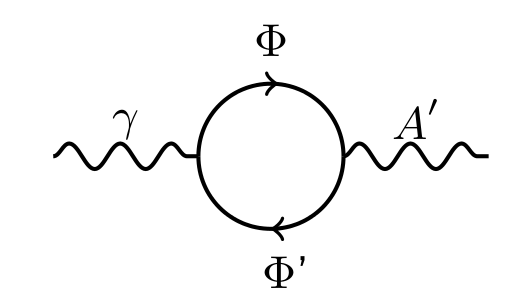
\includegraphics[width=0.5\textwidth]{images/aprime_loop.png}
    \caption{Kinetic mixing of a Standard Model photon with a heavy photon 
    at one-loop through the interaction of massive fields charged under
    the Standard Model hypercharge and dark charge.}
    \label{fig:ap_loop}
\end{figure}
Integrating out the fields generates values of $\epsilon$ on the order of 
\begin{equation}
    \epsilon \sim \frac{g_Yg_D}{16\pi^2}\ln\left(\frac{m_{\Phi}}{m_{\Phi'}} \right)
             \sim 10^{-3} - 10^{-1} 
\end{equation}
where $g_Y$ ($g_D$) are the SM hypercharge (dark) coupling and 
$(m_{\Phi}, m_{\Phi'})$ are the masses of the two fields 
\cite{ArkaniHamed:2008qp, Bjorken:2009mm}.  If the theory doesn't contain 
split multiplets charged under both $U(1)_Y$ and $U(1)'$, the mass splittings 
can be generated by additional loops, leading to values of $\epsilon \sim 10^{-6} - 10^{-3}$. 
In some string theory constructions, 
values as small as $\epsilon \sim 10^{-12}$ are expected 
\cite{Goodsell:2010ie,Goodsell:2009xc, Cicoli:2011yh}.

%
% If I have time, I need to add a paragraph explaining how an A' would acquire
% mass.
%

The possibility that a new gauge boson can couple to charged SM particles is 
very appealing.  It may offer one of the few portals to probe a new sector 
composed of light weakly coupled particles and possibly dark matter
(see section 1.2).  Such a coupling can be exploited by current and future
experimental programs in order to measure the properties of
the hidden sector and possibly provide insight into may outstanding physics puzzles.

\section{Motivations for a Heavy Photon from Dark Matter}

Although the existence of dark matter (DM) has been firmly established through its
gravitational interaction \cite{popolo2014}, its exact nature continues to elude
us. An appealing
possibility is that DM inhabits a ``hidden sector'' with its interactions 
mediated by an $A'$.  In turn, the kinetic mixing of the $A'$ with the SM 
photon may provide a portal that would allow the exploration of not only the 
properties of DM but the hidden sector itself.  Furthermore, several recently
observed astrophysical anomalies \cite{pamela2008, ackermann2012, aguilar2013, 
hooper2011, linden2011, abazajian2012, hooper2013, Bulbul:2014sua}
may have a dark matter interpretation if DM
charge under an $A'$.  A summary of those anomalies along with their dark matter
interpretation will be presented here.

\subsection{Cosmic Rays}

Interest in hidden sector models surged in 2008 with the announcement by 
The Payload for Antimatter Matter Exploration and Light-nuclei Astrophysics \\ 
(PAMELA) of an unforeseen rise in the ratio of the cosmic ray (CR) positron flux
to CR electron flux, $e^{+}/(e^{+} + e^{-})$, above 10 GeV \cite{pamela2008}.
The rise was later confirmed by both the 
Fermi Gamma-Ray Space Telescope \cite{ackermann2012} and Alpha Magnetic 
Spectrometer-02 (AMS-02) \cite{aguilar2013} experiments and observed to continue
up to 200 GeV. 

The main source of CR positrons 
was expected to come from the interaction of CR nuclei with the interstellar 
medium (secondary production).  If such a production mechanism was dominant, 
cosmic ray propagation models predicted the fraction would fall with increasing
energy.  The observed rise lead to the speculation of additional sources of 
positrons including pulsars\cite{yin2013, linden2013}.

One attractive scenario that could account for the rise was the annihilation of
DM to leptons ($e^+e^-, \mu^+\mu^-$). In fact, such models where found to fit 
the data fairly well.  However, such models require much 
larger annihilation rates compared to those expected assuming the typical 
thermal cross-section \cite{Cholis:2008hb}
\begin{equation}
    \left \langle \sigma v \right \rangle \simeq 3 \times 10^{-26} \text{cm}^3 \text{s}^{-1}.
\end{equation}

Alternatively, if DM interactions are mediated by a heavy photon, a 
``Sommerfeld enhancement'' of the annihilation cross-section proportional to
$\sigma v \sim 1/v$ can occur \cite{ArkaniHamed:2008qn}. In such scenarios, the
``freeze-out'' cross-section that leads to the currently observed relic
abundance remain unaffected since the velocity of DM in the early universe was
high and the Sommerfeld enhancement had not effectively turned on.  If the 
heavy photons created in the annihilation of DM subsequently decay to leptons
(Fig. \ref{fig:dm_annihilation}), the resulting $e^+e^-$ spectrum could
account for rise.
\begin{figure}[t]
    \centering
    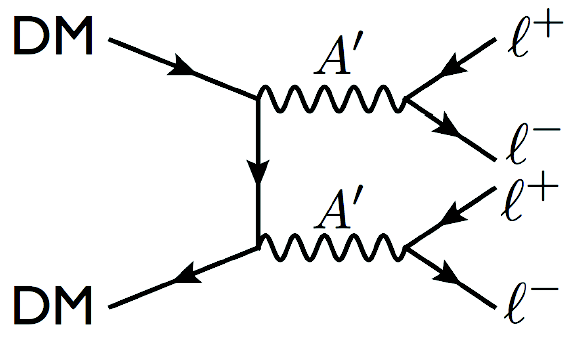
\includegraphics[width=0.5\textwidth]{images/dm_annihilation.png}
    \caption{Dark matter annihilation to a heavy photon which subsequently 
             decays into a pair of leptons.}
    \label{fig:dm_annihilation}
\end{figure}

The most recent measurements of the cosmic microwave background (CMB) have made
it difficult to interpret the positron anomaly as coming from the annihilation
of DM.  
%were to annihilate
%to a heavy photon of mass $\sim$ GeV which subsequently decays to an 
%$e^{+}e^{-}$ 
%the annihilation cross-section of DM at low velocities can be achieved 

%The most recent observations by AMS-02 seem to favor 
%This model became less favorable as higher
%precision measurements of the positron flux became available.  In fact, 
%recent measurements of the cosmic microwave background (CMB) have put very 
%tight constraints on such a scenario.

\subsection{Light Dark Matter}

Recently, an analysis of three years of data collected by the Fermi Large Area
Telescope observed an extended emission in the spectrum of gamma-rays 
originating from the Galactic Center 
\cite{hooper2011, linden2011, abazajian2012, hooper2013}.  Several models have been 
devised to try to explain the emission including the collision of energetic 
protons accelerated by a super-massive black hole \cite{Hooper:2010mq}, 
pulsars \cite{Abazajian:2010zy} and dark matter annihilation to leptons or 
hadron \cite{Hooper:2010mq, Goodenough:2009gk}.  The emission can also
be explained in the context of dark matter annihilating to an $A'$ which 
subsequently decays to SM particles \cite{Hooper:2012cw}.  Such a model assumes
a dark matter candidate of mass $\sim$ 10 GeV annhilating to a heavy photon
with a mass $\sim$ 100 MeV. 

Another anomaly that can be explained in the context of a light dark matter
candidate that couples to a heavy photon is the observance
of a 3.5 keV X-ray line from a 73 galaxy clusters \cite{Bulbul:2014sua}.  
Specifically, the ``eXciting Dark Matter'' model \cite{Finkbeiner:2014sja} 
proposes the existence of a doublet of DM states whose self interactions are 
mediated by a heavy photon. As shown of Figure \ref{fig:dm_self_scat}, a pair
of DM particles upscatter via an $A'$ to produce a pair of excited states, 
$\chi^*\chi^*$. This is immediately followed by the decay 
$\chi^* \rightarrow  \chi\gamma$, producing an X-ray line.
\begin{figure}[t]
    \centering
    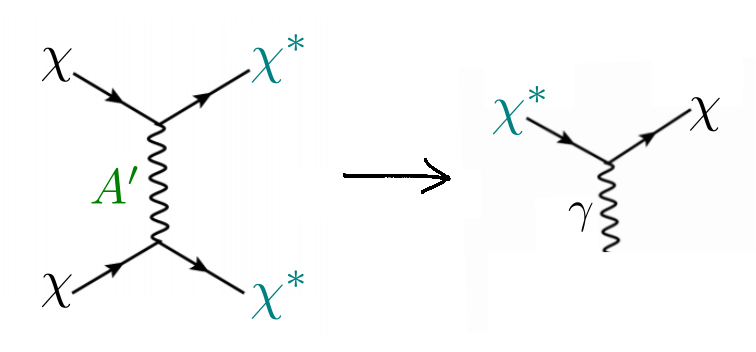
\includegraphics[width=0.9\textwidth]{images/xdm.png}
    \caption{A diagram depicting the self-scattering of dark matter via a heavy
             photon into an excited state. The excited state subsequently decays
             producing an observable X-ray line.}
    \label{fig:dm_self_scat}
\end{figure}


\section{Current Limits on Heavy Photons}
\begin{figure}[ht]
    \centering
    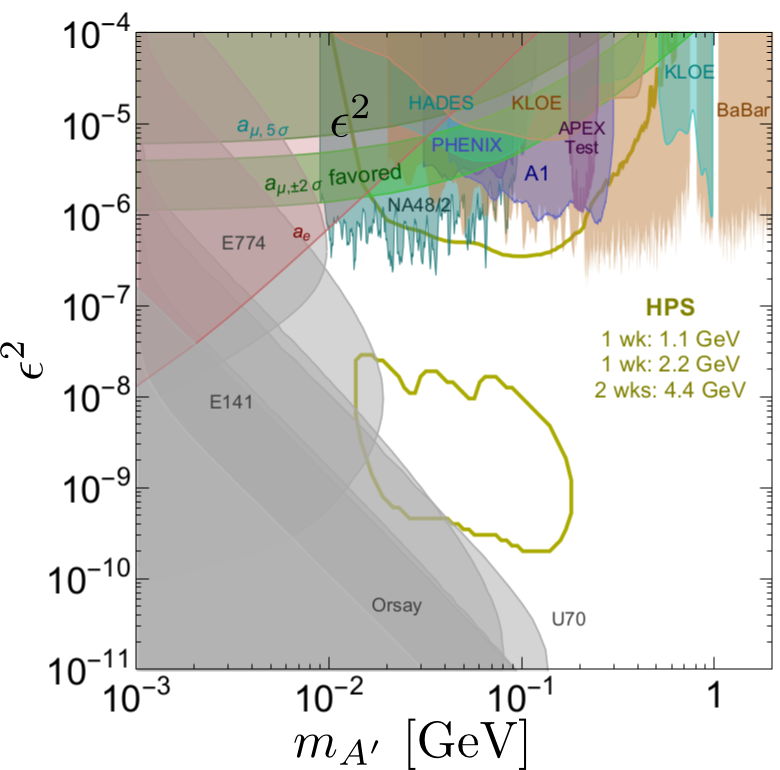
\includegraphics[width=0.9\textwidth]{images/ap_current_limits.png}
    \caption{The estimated 2$\sigma$ reach of the Heavy Photon Search (HPS) 
             experiment along with existing constraints from beam dump  
             \cite{},
             collider \cite{}, 
             and fixed target experiments
             \cite{}.
         The reach calculation assumes HPS running at 1.1 GeV}
    \label{fig:ap_limits}
\end{figure}

\subsection{Electron Beam Dump Experiments}

Electron beam dump experiments make use of a high intensity beam ``dumped'' onto
a thick ($\sim$ cm) target to produce highly boosted heavy photons through a 
process analogous to photon bremsstrahlung.  In order to suppress the large
SM backgrounds produced at the target, a shield of thickness $\sim$ cm - m
is placed immediately downstream, and in front of the detector.  Since the 
heavy photons weakly interact with SM particles, sufficiently long lived 
heavy photons will traverse the shield before reaching an open space upstream
of a detector.  The decay products of heavy photons decaying in this region 
will travel unimpeded until detected.
The thickness of the target and shield in combination with a high luminosity
beam allow such experiments to be sensitive to heavy photons with small 
couplings which tend to travel considerable distances before decaying. Such 
experiments tend to be sensitive to heavy photons with 
$10^{-7} \le \epsilon 10^{-3}$  of masses on the order of 100 MeV. 

% What backgrounds are these experiments concerned with?
% What is the shield made of?

Several electron beam dump experiments were devised over the last several decades with
the intention of searching for axions \footnote{Axions are particles postulated 
by Peccei-Quinn in the last 70's in order to the strong CP problem}.  These 
included E137 \cite{Bjorken:1988as}
and E141 \cite{riordan1987} conducted at SLAC National Accelerator Laboratory,
E774 \cite{bross1991} at Fermi National Accelerator Laboratory, and experiments at 
KEK \cite{konaka1986} in Japan and Orsay \cite{davier1989} in France. 
%The setup of each of the experiments is summarized on Table \ref{}. 
The results from each of these experiments have been reinterpreted in the 
context of a search for a heavy photon and used to set limits on the coupling
strength $\epsilon$ \cite{Bjorken:2009mm, andreas2012}.  The resulting limits are 
shown on Fig. \ref{fig:ap_limits}.

\subsection{Proton Beam Dump Experiments}

Proton beam dump experiments can also be used to search for heavy photons
through either the decay of mesons produced at the target or proton
bremsstrahlung.  The data collected by one such experiment that used the U70
accelerator at IHEP Serpukhov, was originally devised to search for both axions
and a light Higgs boson \cite{Blumlein:1990ay, Blumlein:1991xh}.  The data was 
re-analyzed and a search for an $A'$ was conducted
using the $\pi_0 \rightarrow A'\gamma$ decay channel and proton bremsstrahlung
\cite{johannes2011, johannes2014}. The resulting limits are shown on Fig. 
\ref{fig:ap_limits}.

\subsection{Electron-Positron Colliders}

The past decade saw the operation of several high-luminosity $e^+e^-$ colliders 
that were able to collect a lot of data at different center-of-mass energies.
These include KLOE running at the the DA$\Phi$NE $\phi$ factory and BaBar, 
at the PEP-II B-Factory. Searches at BaBar were performed using the channel 
$e^+e^- \rightarrow A' \gamma (A' \rightarrow \mu^+\mu^-)$ 
\cite{Reece:2009un, Aubert:2009cp}.  KLOE 
searched for heavy photons in the decays of the $\phi$ meson.  Specifically, 
the channel $\phi \rightarrow \eta A' (A' \rightarrow e^+e^-)$ was used to
set limits on the coupling strength of the $A'$ 
\cite{Babusci:2012cr, Archilli:2011zc}.
The limits set by both BaBar and KLOE are shown on Fig. \ref{fig:ap_limits}.

\subsection{Electron Fixed Target Experiments}

\section{The Heavy Photon Search Experiment}



%%%%%%%%%%%%%%%%%%%%%%%%%%%%%%%%%
%  HPS Signal and Backgrounds   %
%%%%%%%%%%%%%%%%%%%%%%%%%%%%%%%%%

\chapter{HPS Signal and Backgrounds}

The Heavy Photon Search is a fixed target experiment that will search for heavy
photons in the mass range of 20 MeV/c$^{2}$ to 500 MeV/c$^{2}$ and couplings
of $\epsilon \sim 10^{-5} - 10^{-10}$.  Since heavy photons couple to electric
charge, they can be produced by a process analogous to bremsstrahlung 
radiation.  The heavy photon subsequently decays to narrow $e^+e^-$ resonances, 
which can be observed above the dominat quantum electrodynamic (QED) trident
background.  For suitably small couplings, heavy photons travel detectable 
distances before decaying providing a second signature.  In the chapter that
follows, both the heavy photon production mechanism and background involved 
in such a search will be discussed.

\section{Heavy Photon Production}

Sensitivity to the theoretically favored regions of the heavy photon 
mass-coupling phase space can be best achieved using high luminosity fixed
target experiments \cite{PhysRevD.80.075018}.  In such experiments, an electron
of energy $E_{0}$ incident on a high $Z$ target will radiate heavy photons 
through a process analogous to ordinary photon bremsstrahlung.  The differential
(Fig. \ref{fig:ap_production}).  
\begin{figure}[t]
    \centering
    \caption{A' being produced.}
    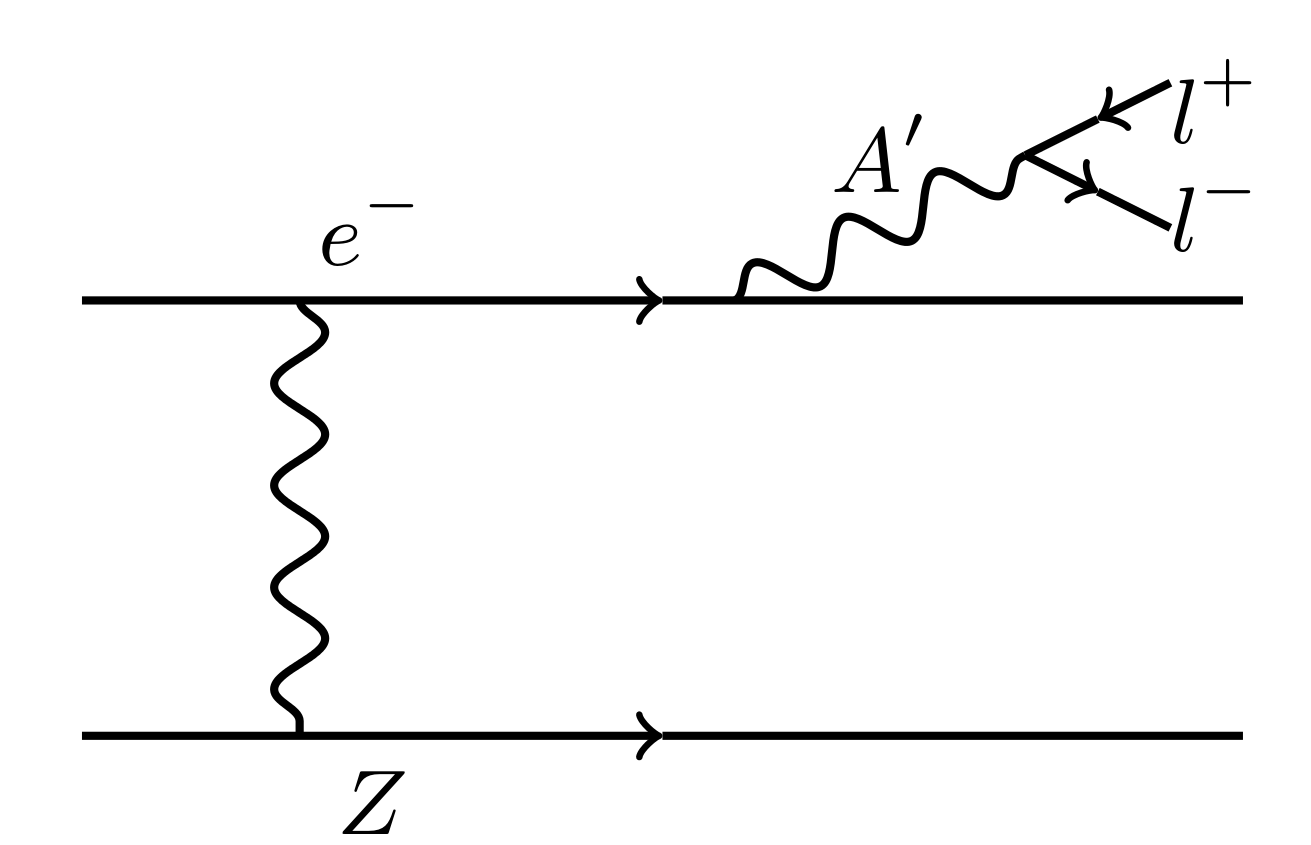
\includegraphics[width=0.5\textwidth]{images/aprime_brem.png}
    \label{fig:ap_production}
\end{figure}  
cross-section of such a process can be estimated using the Weizacker-Williams 
approximation as 
\[
    \frac{\sigma}{dx d\cos{\theta_{A}}} \approx \frac{8 Z^{2} \alpha^{3} \epsilon^{2} E_{0}x}{U^{2}} \chi
            \time [(1 - x + x^{2}/2) - x(1-x)m_{A'}^{2}E_{0}^{2}x\theta_{A'}^{2}/U^{2}]
\]
where $\alpha \sim 1/137$ is the fine structure constant, $\theta_{A}$ is the 
scattering angle of the $A'$, $\chi$ is the effective photon flux and 
\[
    U(x, \theta_{A'}) = E_{0}^{2}x\theta_{A'}^{2} + m_{A'}^{2}\frac{1-x}{x} + m_{e}^2 x
\]
is the virtuality of the intermidiate electron.

%In the case that the mass of the heavy photon is zero, equation
Although heavy photons are produced in a process similar to ordinary bremsstrahlung, 
their production rate and kinematics differ in several ways: 
\begin{itemize}
    \item The production cross-section is suppressed by a factor of $\epsilon^{2}m_{e}^{2}/m_{A'}^{2}$.
    \item The $A'$ is produced very forward.
    \item The $A'$ will take most of the incident beam energy.
\end{itemize}

\section{Trident Backgrounds}

The primary background expected to dominate the final event sample of the Heavy
Photon Search experiment is the quantum electrodynamic Trident process.  As 
shown on Fig. (), the tridents can be seperated out into two main diagrams: 
\begin{figure}[t]
    \centering
    \caption{A' being produced.}
    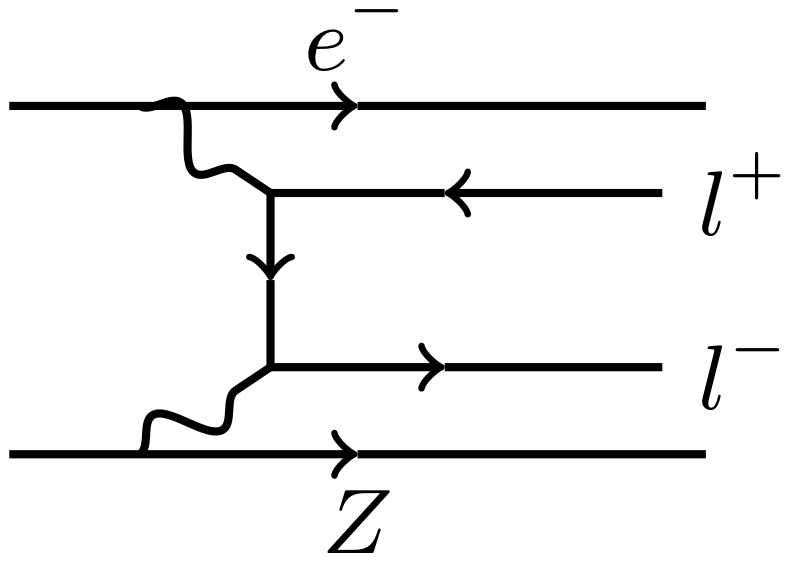
\includegraphics[width=0.5\textwidth]{images/bethe-heitler.png}
    \label{fig:tridents}
\end{figure}  
Bethe-Heitler and radiatives. The kinematics of radiativesare indistinguishable
from the $A'$ signal events within an invariant mass window near the $A'$ mass.
Therefore, radiatives can be used to analyze both the rate of the $A'$ signal 
production and the sensitivity of an experiment to $A'$ signals.  Specifically,
the $A'$ production cross-section is related to the production cross-section of 
radiatives as 
\[
    \frac{d\sigma(A')}{d\sigma(\gamma^*)} = \frac{3\pi\epsilon^{2}}{2 N_{eff} \alpha}
        \frac{m_{A'}}{\delta m}
\]
As a result, the radiatives in the final event sample can be used to analyze 
the $A'$.

Although the rate of the Bethe-Heitler process dominates among the two processes, 
its different kinematics can be used to reduce them in the final event sample.
Specifically, the $A'$ decay products are highly boosted while the recoiling 
electron is soft and scatters at large angles.  In contrast, at higher 
energies, the Bethe-Heitler process is not enhance.  Furthermore, only one of
the leptons in the pair will be highly boosted, while the other will be much
softer.  The recoiling electron will be produced much more forward.




%%%%%%%%%%%%%%%%%%%%%
%   HPS Apparatus   %
%%%%%%%%%%%%%%%%%%%%%

\chapter{The HPS Apparatus}

%The HPS experiment engineering run was conducted in the Spring of 2015 at the
%Thomas Jefferson National Accelerator Facility (JLab) in Newport News, VA.  The
%HPS detector was installed within the Hall B alcove upstream of the Continuous 
%Electron Beam Accelerator Facility (CEBAF) Large Acceptance Spectrometer for 12
%GeV (CLAS12) detector.  HPS utilized CEBAF's high luminosity electron beam,
%operating at an energy of 1.056 GeV and current of 50 nA, incident on a thin
%(~0.125\% $X_{0}$) tungsten target to search for an $A'$ with a mass in the 
%range of 20 - 100 MeV.  

At the energies at which the HPS experiment is operating, the 
electroproduced $A'$ will carry most of the incident beam energy. Consequently,
the $A'$ decay products will be highly boosted, necessitating a detector with very
forward acceptance that can be placed in close proximity to the target.
Maximizing the acceptance requires placing the detector close to the beam plane,
encroaching on a ``dead zone'' which is occupied by an intense flux of multiple
Coulomb scattered beam particles along with radiative secondaries originating
from the target.  In order to avoid additional background from from beam gas
interactions, the detector needs to operate in vacuum. Finally, minimizing the
material budget of the active area of the detector is essential to reducing the
multiple scattering that dominates both the mass and vertex resolutions that
determine the experimental sensitivity.

These design principles led to the conception of the HPS detector.  
Specifically, HPS utilizes a compact, large acceptance forward spectrometer 
consisting of a silicon microstrip tracker (SVT) along with a lead tungstate
electromagnetic calorimeter (Ecal).  The SVT is installed inside of a vacuum
chamber and inside of an analyzing magnet immediately downstream of a thin
($0.125\%X_{0}$) tungsten target.
The Ecal is placed downstream of the tracker and provides the primary 
trigger for the experiment and is also used for electron identification. Together, 
both subsystems provide the complete kinematic information required to 
reconstruct heavy photons.

The HPS detector was installed and commissioned within the Hall B alcove at the
Thomas Jefferson National Accelerator Facility (JLab) in Newport News, VA early
in the Spring of 2015. Shortly after, an engineering run took place utilizing
the Continuous Electron Beam Accelerator Facility (CEBAF) operating at an 
energy 1.056 GeV and current of 50 nA.

The chapter that follows will detail various elements of the experiment.
It will begin with a discussion of CEBAF and continue with descriptions
of several beamline elements, SVT, Ecal and data acquisition system (DAQ).

\section{CEBAF}

CEBAF's ability to provide a nearly continuous, clean and intense electron
beam makes it ideal to search for heavy photons with weak couplings. Recently,
CEBAF underwent an upgrade that increased its maximum operating energy to 12
GeV and introduced a new experimental hall, Hall D, that will house the
GlueX detector \cite{Dudek:2012vr}.  The upgraded facility is now capable of 
delivering 11 GeV electron beams to the three existing experimental halls
(Hall A, B, C) and can use the 12 GeV electron beam to generate and deliver a 9
GeV photon beam to Hall D. 

As shown on Figure \ref{fig:cebaf}, achieving 12 GeV operation, required several
improvements to the accelerator \cite{Burkert:2012rh}. Central to the upgrade 
was the addition of 5 
cryomodules to each of the linacs.  Coupled with upgrades to the accelerator
magnets and power supplies, the additional cryomodules allowed each linac to
accelerate electrons at a rate of 2.2 GeV per pass up to a maximum of 5 passes.
\begin{figure}[h]
    \centering
    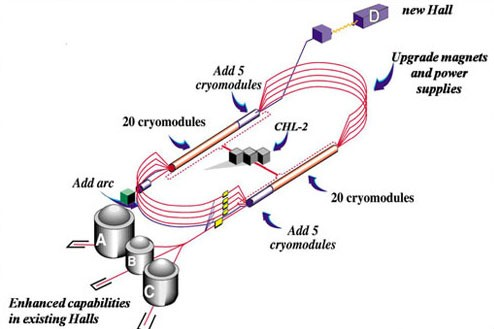
\includegraphics[width=0.9\textwidth]{images/cebaf.jpg}
    \caption{A diagram of the Thomas Jefferson National Accelerator Facility
             Continuous Electron Beam Accelerator Facility showing the 
             components that were upgraded as part of the 12 GeV Upgrade 
             program.}
    \label{fig:cebaf}
\end{figure}
Enabling four hall operation also required the addition of a new 750 MHz RF 
separator, a new laser to the electron source and a 10th arc which provides
the additional pass of acceleration that allows 
delivery of the maximum beam energy to Hall D.


\subsection{Electron Production and Injection}

%
%  Note: I need to make sure that this is still correct in the 12 GeV era.
%
The electrons injected into the accelerator were produced by photoemission from
a strained GaAs superlattice photocathode \cite{Maruyama:2004hx}.  Each of the 
four experimental halls has a dedicated gain-switched fiber coupled laser of
wavelength 1560 nm.  The lasers are frequency doubled in order to produce light
of wavelength of 780 nm, matching the band gap of the superlattice cathode. The
lasers are phased shifted and are each pulsed for $\approx$ 40 ps at the 
frequency of 499 MHz.  Since the operational frequency of the accelerator 
cryomodules is 1497 MHz, four hall operation requires subharmonics of 499 MHz to
be chosen.  This is achieved by ``cutting away'' pulses using an optical 
modulator \cite{Kazimi:2013yua}.


The photoemission electrons are released into an extremely high vacuum
environment at a pressure of $10^{-11}$ to $10^{-12}$ Torr.  The free electrons
are then delivered into the injector by a 100 keV electron gun.  The injector
itself then accelerates the electron bunches to an energy of 50 MeV 
%by 2 1/4 cryomodules 
before being delivered into the accelerator.

\subsection{Electron Acceleration}

The CEBAF accelerator is composed of two linacs arranged in a racetrack
configuration as shown on Fig \ref{fig:cebaf}. Each of the linacs consist
of 25 cryomodules, 5 of which were added as part of the upgrade.  The original
(new) cryomodules consist of 8 5-cell (7-cell) superconducting radio frequency
(RF) cavities made of ultra-pure Niobium (see Figure \ref{fig:cebaf_cavity}).  
The original cryomodules
\begin{figure}[h]
    \centering
    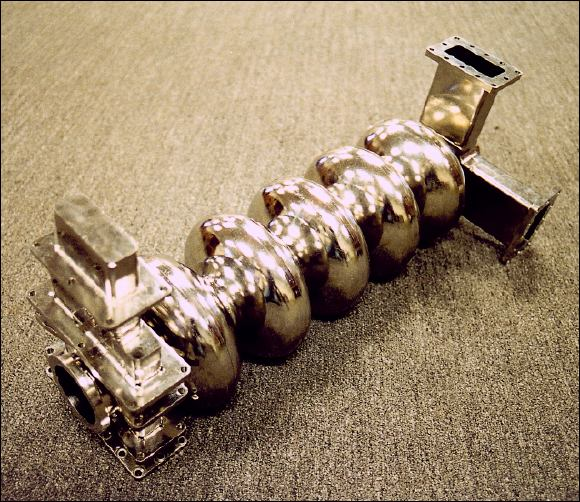
\includegraphics[width=0.7\textwidth]{images/cebaf_cavity.jpg}
    \caption{A 5-cell ultra-pure Niobium superconducting radio frequency cavity
             used to accelerate electrons at CEBAF.}
    \label{fig:cebaf_cavity}
\end{figure}
are capable of accelerating an electron upwards of 25 MeV while the newly installed
cryomodules can achieve an acceleration of 100 MeV.  This leads to an acceleration
of 1.1 GeV per linac and 2.2 GeV per pass. The 
number of passes depends on the energy requirements of the experiment taking place.
However, for electrons delivered to Halls A, B and C, the maximum amount of passes
is 5 while for Hall D, it's 5.5.

Electron bunches circulating the accelerator can be delivered to a Halls A, B
and C by an RF separator operating at a frequency of 499 MHz.  Delivery to Hall
D uses an RF separator of 750 MHz.

\subsection{Single Pass Operation For HPS}

During the Spring of 2015, HPS was prepared to run at a beam energy of 2.2 GeV,
in conjuction with the commissioning of the 750 MHz RF separator.
Unfortunately, an incident occurred which resulted in the loss of the new CHL
required to operate the accelerator as a 12 GeV machine.
The loss caused the accelerator to 
fallback to 6 GeV operation using a single CHL.  As a result, HPS was given
the unique opportunity to run with a beam energy of 1.056 GeV allowing the
experiment to have sensitivity to the g-2 favored region of the mass-coupling
phase space.  

\section{Beamline}

\subsection{Layout}

The HPS experiment is installed within the Hall B alcove and utilizes a 
three-magnet chicane system as shown on Figure \ref{fig:beamline}. 

\subsection{Beam Quality}

In order to optimize the ve





%The first and last dipoles of the chicane,  are used to bend
%the beam into the HPS apparatus while the second dipole, the Hall B pair 
%spectrometer, serves as the analyzing magnet of the experiment.  

\begin{sidewaysfigure}
    \centering
    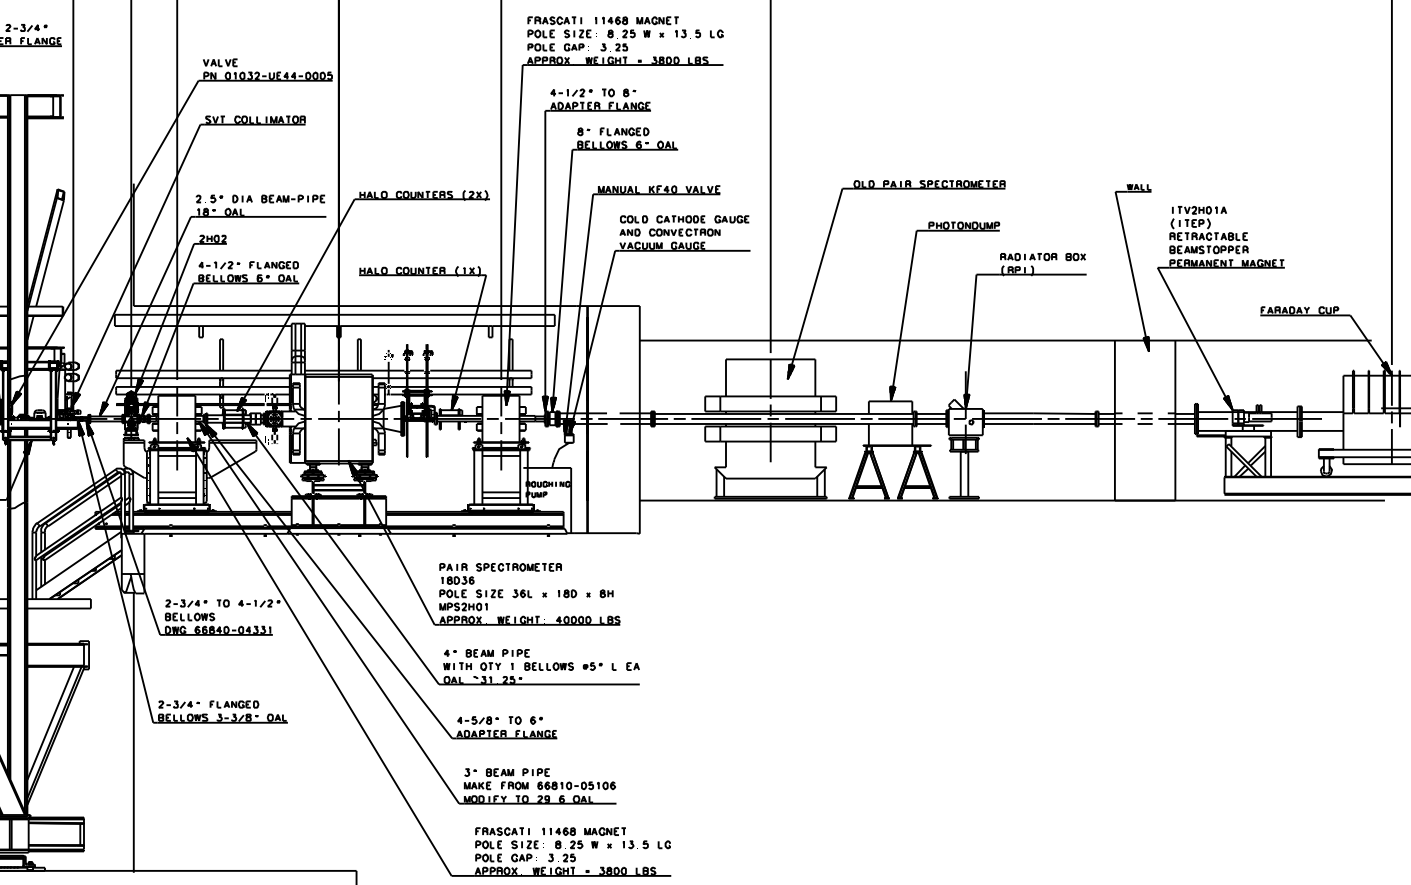
\includegraphics[width=\textwidth]{images/beamline.png}
    \caption{Configuration of the beam line during the HPS engineering run.}
    \label{fig:beamline}
\end{sidewaysfigure}

\section{Silicon Vertex Tracker}

\subsection{Layout}

The HPS SVT is comprised of two halves of six measurement layers encroaching the
beam plane as shown of Figure \ref{fig:svt_layout_render}. Each layer consist of a pair of
closely-spaced silicon planes with one of the planes oriented orthogonal to
the beam plane and the other at small angle stereo 
(see Table \ref{tab:svt_layout}).
\begin{figure}[h!t]
    \centering
    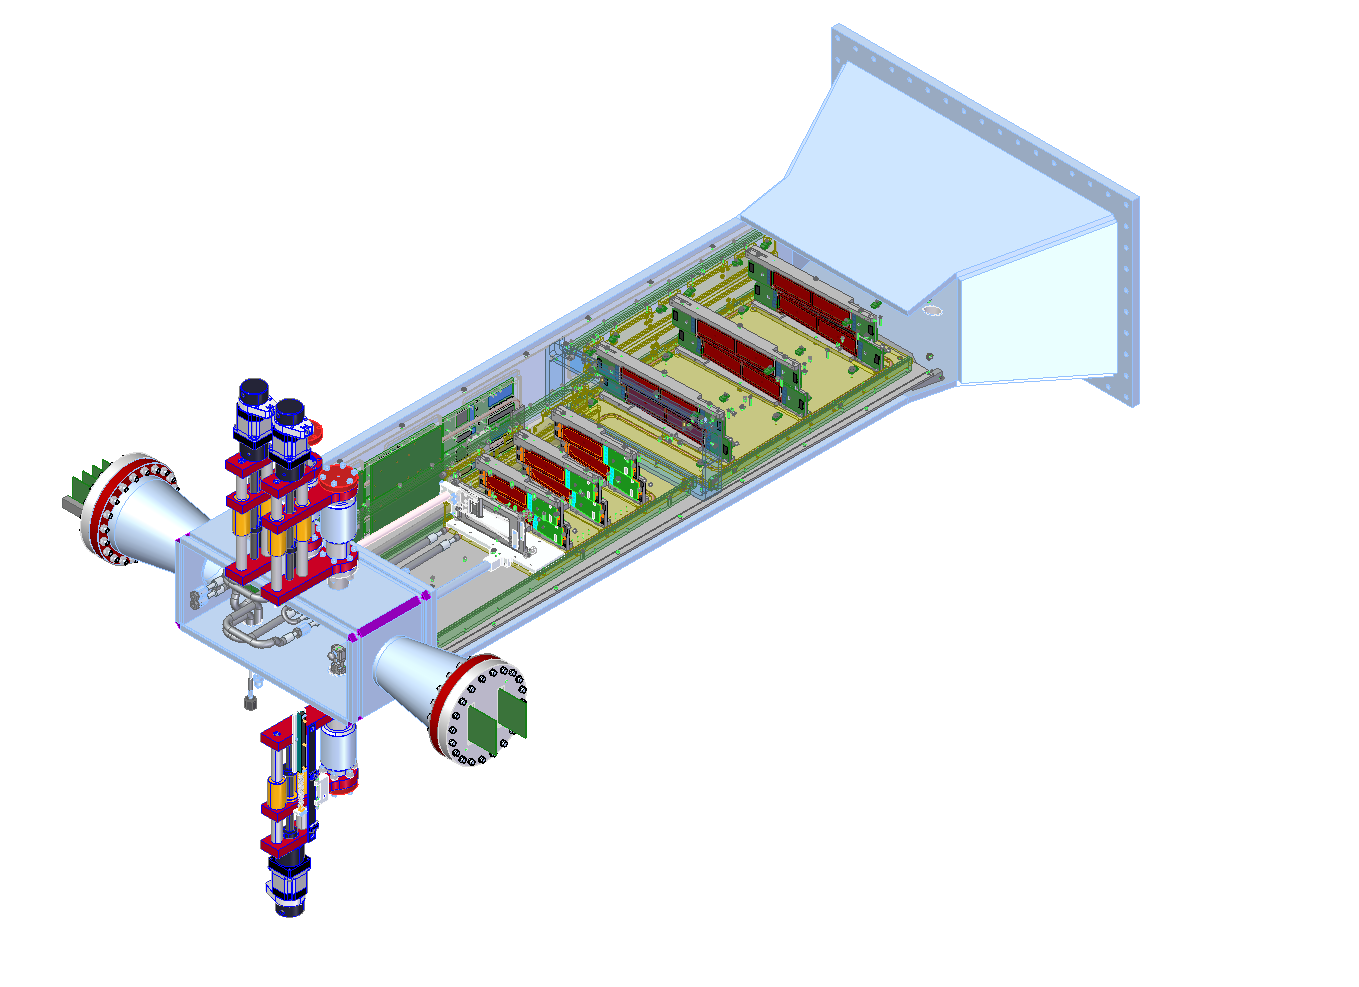
\includegraphics[width=0.9\textwidth]{images/svt_layout_render.png}
    \caption{A rendered view of the Silicon Vertex Tracker inside of the pair
             spectrometer vacuum chamber.}
    \label{fig:svt_layout_render}
\end{figure}
This allows
for the measurement of both the vertical and horizontal coordinate of a hit, in turn, 
enabling full 3D hit reconstruction.  

The first three layers consist of a single sensor of coverage above and below
the beam plane and use a stereo angle of 100 mrad. In order to better match the
% needs a sentence explaining why 100 mrad stereo was used.  According to the
% proposal, it balances acceptance against vertexing resolution.
acceptance of the Ecal, the coverage of the last three layers is two sensors 
wide and use a stereo angle of 50 mrad.  The choice of a 50 mrad angle for the
last three layers instead of 100 mrad was meant to break the degeneracy that
results in fake tracks
due to ghost hits in layers with the same stereo angle.  It must be noted that
only five layers are needed to match the full acceptance of the Ecal, however,
an improvement in the momentum resolution was observed with the addition of 
another layer.  In total, the SVT makes use of 36 sensors, which amounts to 
23,004 channels.

Since heavy photons are produced very forward, and the opening angle of their 
decay products goes as $\sim m_{A}/E_{0}$, sensitivity to low mass heavy photons
requires
the tracker layers to be as close to the beam plane as possible.  When deciding
the distance of the first layer to the beam, several effects needed to be taken
into consideration. These include the extent of the beam halo, the amount of 
radiation damage that is expected to be incurred from the Coulomb scattering
of the primary beam as well as radiative secondaries, the ability to resolve 
hits with pileup present and being capable of doing pattern recognition in a high 
occupancy environment.  With all of this in mind, it was determined that the 
closest tolerable distance was 15 mrad, putting the active edge of layer 1 
at 0.5 mm from the beam center. In simulation, this corresponds to 1\% occupancy
of strips closest to the beam plane of layer 1.

% I should talk about the positions as surveyed.
%The SVT layout is summarized in Table \ref{tab:svt_layout}. \textbf{Talk about
%the survey}.

%%%%%%%%%%%%%%%%%%%%%%%%%%%
%%% Table of SVT layout %%%
%%%%%%%%%%%%%%%%%%%%%%%%%%%
% I should use the survey positions here.
%\begin{table}[t]
\begin{sidewaystable}
    \centering
    \begin{tabular}{lcccccc}  
        \toprule
        \textbf{Layer} & \textbf{1} & \textbf{2} & \textbf{3} & \textbf{4} & \textbf{5} & \textbf{6} \\
        \midrule
        \midrule
        $z$ position from target (cm)    & 10 & 20 & 30 & 50 & 70 & 90 \\
        Stereo angle (mrad) & 100 & 100 & 100 & 50 & 50 & 50 \\
        Bend plane resolution ($\mu$m) & $\approx$6 & $\approx$6 & $\approx$6 & $\approx$6 & $\approx$6 & $\approx$6 \\
        Non-bend plane resolution ($\mu$m) & $\approx60$ & $\approx60$ & $\approx60$ & $\approx120$ & $\approx120$ & $\approx120$ \\
        Nominal dead zone in $y$ (mm) & $\pm$ 1.5 & $\pm$ 3.0 & $\pm$ 4.5 & $\pm$ 7.5 & $\pm$ 10.5 & $\pm$ 13.5 \\ 
        Material budget & .7\% & .7\% & .7\% & .7\% & .7\% & .7\% \\
        \bottomrule
    \end{tabular}
    \caption{The layout of the HPS SVT.}
    \label{tab:svt_layout}
\end{sidewaystable}
%%%%%%%%%%%%%%%%%%%%%%%%%%%

\subsection{Sensors}

At the energies at which HPS operates, the uncertainty in both the mass and
vertex resolutions are dominated by multiple Coulomb scattering in the first 
few layers.  This made it important to choose a sensor technology that would 
minimize the material budget of the SVT modules, especially since the material
budget of the sensors dominates the total material budget of the SVT modules.
Furthermore, the need to place the SVT in close proximity
to the beam plane made it necessary to choose sensors which are highly tolerant
to radiation.  With these 
considerations in mind, a readily available batch of silicon microstrip sensors,
initially manufactured for the D0 Run IIb upgrade, were found to satisfy all 
necessary requirements \cite{D0Collab:2003}.

The sensors were manufactured by Hamamatsu Photonics Corporation on 
$\langle 100 \rangle$ crystal rotation silicon and are $p^{+}$ on $n$-bulk, 
single sided, AC-coupled and polysilicon-biased. The cut dimensions of the 
sensors are $100 \times 40.34$ mm$^{2}$ with an active area of 
$98.33 \times 38.34$ mm$^{2}$. They are $320 \pm 20 \mu$m thick and have a sense
(readout) pitch of 30 (60) $\mu$m. The sensor specifications are summarized on 
Table \ref{tab:sensor_specs}.
\begin{table}[t]
    \centering
    \begin{tabular}{lr}
        \toprule
        Cut dimensions (L$\times$W)     & 100 mm x 40.34 mm \\
        Active area (L$\times$W)        & 98.33 mm x 38.34 mm \\
        Readout (Sense) pitch           & 60 (30) $\mu$m \\
        \# Readout (Sense) strips       & 639 (1277) \\
        Breakdown voltage               & $>1000$ V \\
        Depletion voltage               & $> 130$ V \\
        Bias Resistor Value             & $0.8 \pm 0.3$ M$\Omega$ \\
        AC Coupling Capacitance         & $>12$ pF/cm \\
        Total Interstrip Capacitance    & $< 1.2$ pF/cm \\
        Defective Channels              & $<1$ \% \\
        \bottomrule
    \end{tabular}
    \caption{Specifications of the sensors used for the HPS SVT.}
    \label{tab:sensor_specs}
\end{table}

Over the lifetime of the HPS detector, the sensor strips closest to the beam 
plane are expected to see $>10^{15}$ electrons per cm$^2$.  The radiation
damage the sensors are expected to incur due to the large electron flux,
will lead to an increase in both the leakage current and the voltage required to 
fully deplete the sensor.  It was then beneficial to choose a sensor technology
that can be operated at high bias voltage in order for them to remain fully
depleted even after irradiation. In fact, previous studies have shown that 
sensors that may be operated to 1000 V can tolerate a dose of 
$1.5 \times 10^{14}$ 1 MeV neq/cm$^2$ \cite{Fretwurst:2002vb}.  Since the damage
incurred by electrons with energies less than 10 GeV is a factor $\sim$ 30 less
than 1 MeV neutrons \cite{Rashevskaya:2002nd},
then ensuring all sensors can be biased to 1000 V will ensure that the sensors
will be able to withstand the expected flux of electrons over the lifetime of
HPS. 


Before being considered for use for the SVT modules, all sensors were electrically 
characterized.  Specifically, the leakage current was measured as a function
of bias voltage up to a maximum bias of 1000 V.  During these test, leakage 
currents of less than 500 nA were observed.  The measured IV curves for a subset
of sensors can be seen on Fig. \ref{fig:sensor_iv_curves}.  Only sensors whose
leakage current did not uncontrollably increase (i.e. breakdown) before reaching
a bias of 1000 V  were considered for use in HPS.
\begin{figure}[t!]
    \centering
    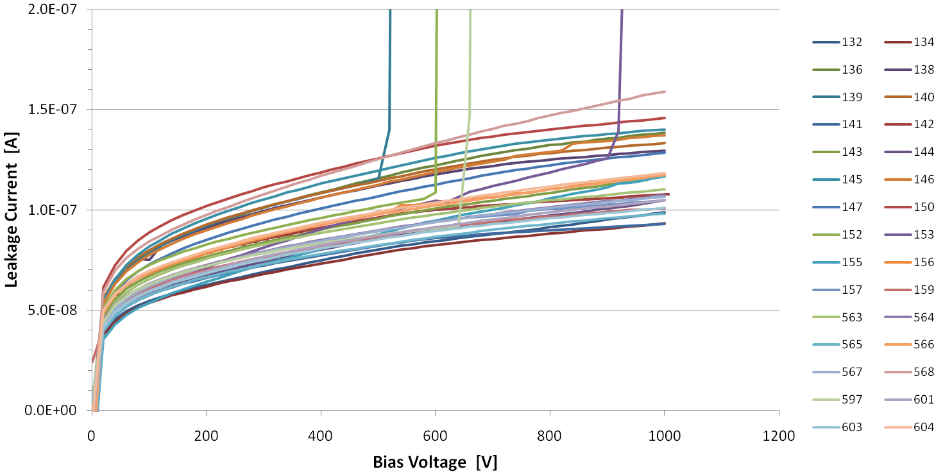
\includegraphics[width=\textwidth]{images/sensor_iv_curves.png}
    \caption{Measured IV curves for a subset of sensors used by HPS.}
    \label{fig:sensor_iv_curves}
\end{figure}

\subsection{Readout} \label{subsec:readout}

The sensors are continuously read out using the APV25 readout chip developed for
the Compact Muon Solenoid detector at the Large Hadron Collider 
\cite{Raymond:2000ey}. The APV25 has 128 channels, with each channel consisting
of a charge sensitive pre-amplifier coupled to CR-RC shaping amplifier and a 192
cell deep analog pipeline.  A schematic of a single channel is shown on 
Fig. \ref{fig:apv25_schem}.
\begin{figure}
    \centering
    \includegraphics[width=\textwidth]{images/apv25_channel_schematic.png}
    \caption{A schematic of a single channel of the APV25 readout chip.}
    \label{fig:apv25_schem}
\end{figure}

When a particle traverses a sensor, it generates a charge signal which is 
processed by the APV25 amplifier chain.  As shown on Figure 
\ref{fig:apv25_pipeline}, the shaper
\begin{figure}
    \centering
    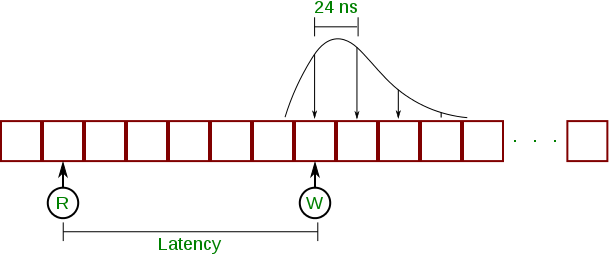
\includegraphics[width=\textwidth]{images/apv25_pipeline.png}
    \caption{A schematic demonstrating the sampling of the shaper signal and
             the management of read/write pointers.}
    \label{fig:apv25_pipeline}
\end{figure}
output is continuously sampled at 41.6 MHz into the analog pipeline. The position
along the pipeline into which the shaper output is stored is determined by 
a write pointer which continuously cycles the pipeline.  Similarly, a read 
pointer determines the position that will be marked for read out when a trigger
signal is received.  Since the trigger decision cannot happen instantaneously,
the distance between the read and write pointers or latency is programmable.
Given that only 160 pipeline cells out of the 192 are used
to buffer samples, the delay between a signal and the arrival of the trigger can
be as long as 3.8 $\mu s$. The remaining 32 cells along the pipeline are used 
to buffer the addresses of samples that are waiting to be read out.

The samples  are readout out by the Analog Pulse Shape Processor (APSP) which
can operate in two modes: peak and deconvolution mode.  In peak
mode, only a single pipeline cell is read out corresponding to the maximum 
value of the shaper output.  In deconvolution mode, three consecutive samples are
read out allowing for the reconstruction of the shaper output.  The output of 
the APSP is then sent to a 128:1 multiplexer which then makes the raw data 
frames. 
%An example of the output data frame is shown on Figure \ref{}.

During the engineering run, the APV25s were operated using the nominal settings
with listed on Table \ref{tab:apv_specs}.  At nominal, the shaping time is set
to 50 ns.  The high occupancies expected during the engineering
run meant that overlapping of hits or ``pile-up'' were a concern.  In order to 
mitigate this problem, the APV25's were operated in deconvolution allowing 
the reconstruction of the shaper output.  Furthermore, 
with each Ecal trigger, the APV25's were sent two consecutive trigger signals 
allowing the readout of six consecutive samples instead of three.  The trigger
latency was then adjusted such that two samples before the signal were readout, 
allowing the shape of the pileup pulse to be captured by the fit.  This was 
used to remove any effects of pileup from the signal pulse.  Approximately 5\%
of hits in layer were observed to be affected by pileup.
\begin{table}[ht]
    \centering
    \begin{tabular}{llr}
        \toprule
        \textbf{Name} & \textbf{Description} & \textbf{Value} \\
        \midrule
        \midrule
        IPRE   & Preamp input FET current       & 98 (460 $\mu$A)\\
        IPCASC & Preamp cascode current         & 52 (60 $\mu$A) \\
        IPSF   & Preamp source follower current & 34 (50 $\mu$A) \\
        ISHA   & Shaper input FET current bias  & 34 (50 $\mu$A) \\
        ISSF   & Shaper source follower current & 34 (50 $\mu$A) \\
        IPSP   & APSP current                   & 55 (80 $\mu$A) \\
        IMUXIN & Multiplexer input current      & 34 (50 $\mu$A) \\
        VFP    & Preamp feedback voltage        & 30  \\
        VFS    & Shaper feedback voltage        & 60  \\
        VPSP   & APSP Voltage level             & 40  \\
        LATENCY & Trigger latency               & 147 \\
        MUXGAIN & Multiplexer gain              & 100 $\mu$A/MIP \\
        \bottomrule
    \end{tabular}
    \caption{APV25 specs used during the engineering run.}
    \label{tab:apv_specs}
\end{table}
%\ref{fig:apv_shape}.
%\begin{figure}
%    \centering
%    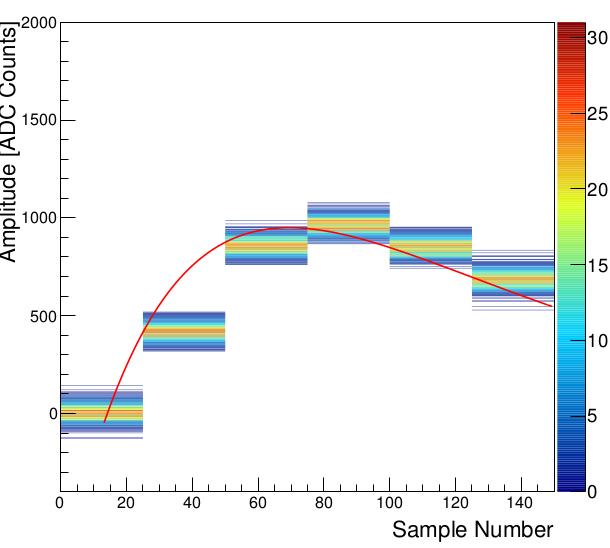
\includegraphics[width=0.9\textwidth]{images/sideB_response_ch535.png}
%    \caption{The signal shape observed during the engineering run.}
%    \label{fig:apv_shape}
%\end{figure}

\subsection{SVT Modules}

Each of the layers of the SVT consist of a ``module'' built by placing
two ``half-modules'' back-to-back around an aluminum cooling block.  The 
half-modules used for layers 1-3 are composed of a single sensor
and FR4 hybrid electronic board glued onto a polyimide-laminated carbon fiber
composite backing.  In order to better match the acceptance of the Ecal, 
the half-modules used in layers 4-6 consist of two sensors glued end-to-end onto
the polyimide-laminated carbon fiber backing with hybrids on either side of them.


%Due to space constraints, the hybrids used
%by layers 4-6 have smaller footprint.  In order to further minimize the 
%amount of material, a window is machined in the carbon fiber leaving the middle
%of the sensor exposed. Fig. \ref{fig:l13_hm} and \ref{fig:l46_hm} show both a layer 1-3 and 4-6 
%half-modules.


%Reading out of a sensor requires the use of 5 APV25 chips.


%An SVT ``half-module'' consist of an electronic readout board, 



%Each sensor requires 5 APV25 chips in order to readout all channels.  The 5 
%APV25 chips are mounted on a FR4 electronic readout board, or hybrid, containing
%filtering for the high voltage bias and a temperature sensor.  Since the pitch
%of the APV25 and the sensors are similar, the chips were wirebonded directly to
%the sensors without the need of a pitch adapter.

\begin{figure}
    \centering
    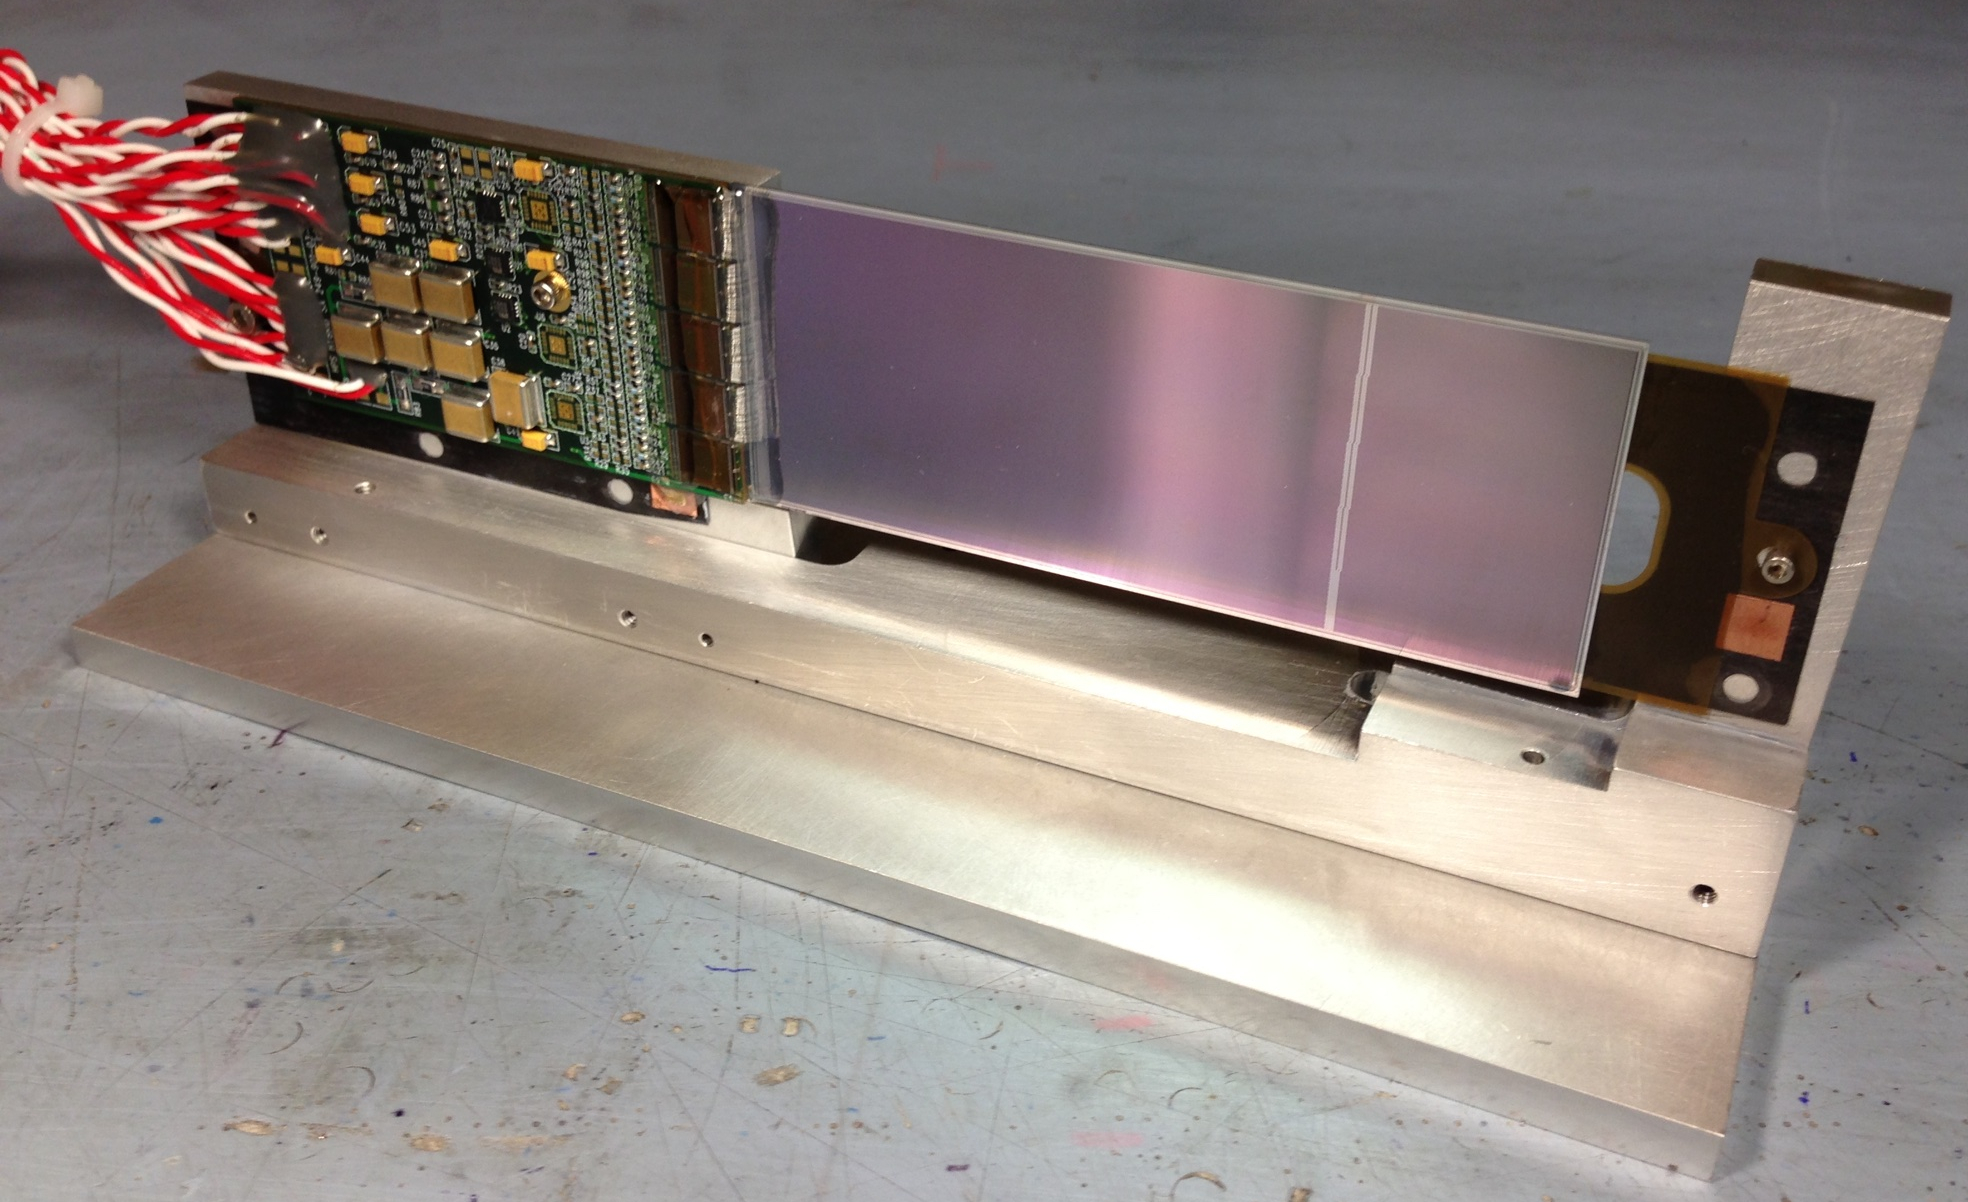
\includegraphics[width=0.9\textwidth]{images/l13_half_module.jpg}
    \caption{A layer 1-3 half-module used by the SVT. }
    \label{fig:l13_hm}
\end{figure}
\begin{figure}
    \centering
    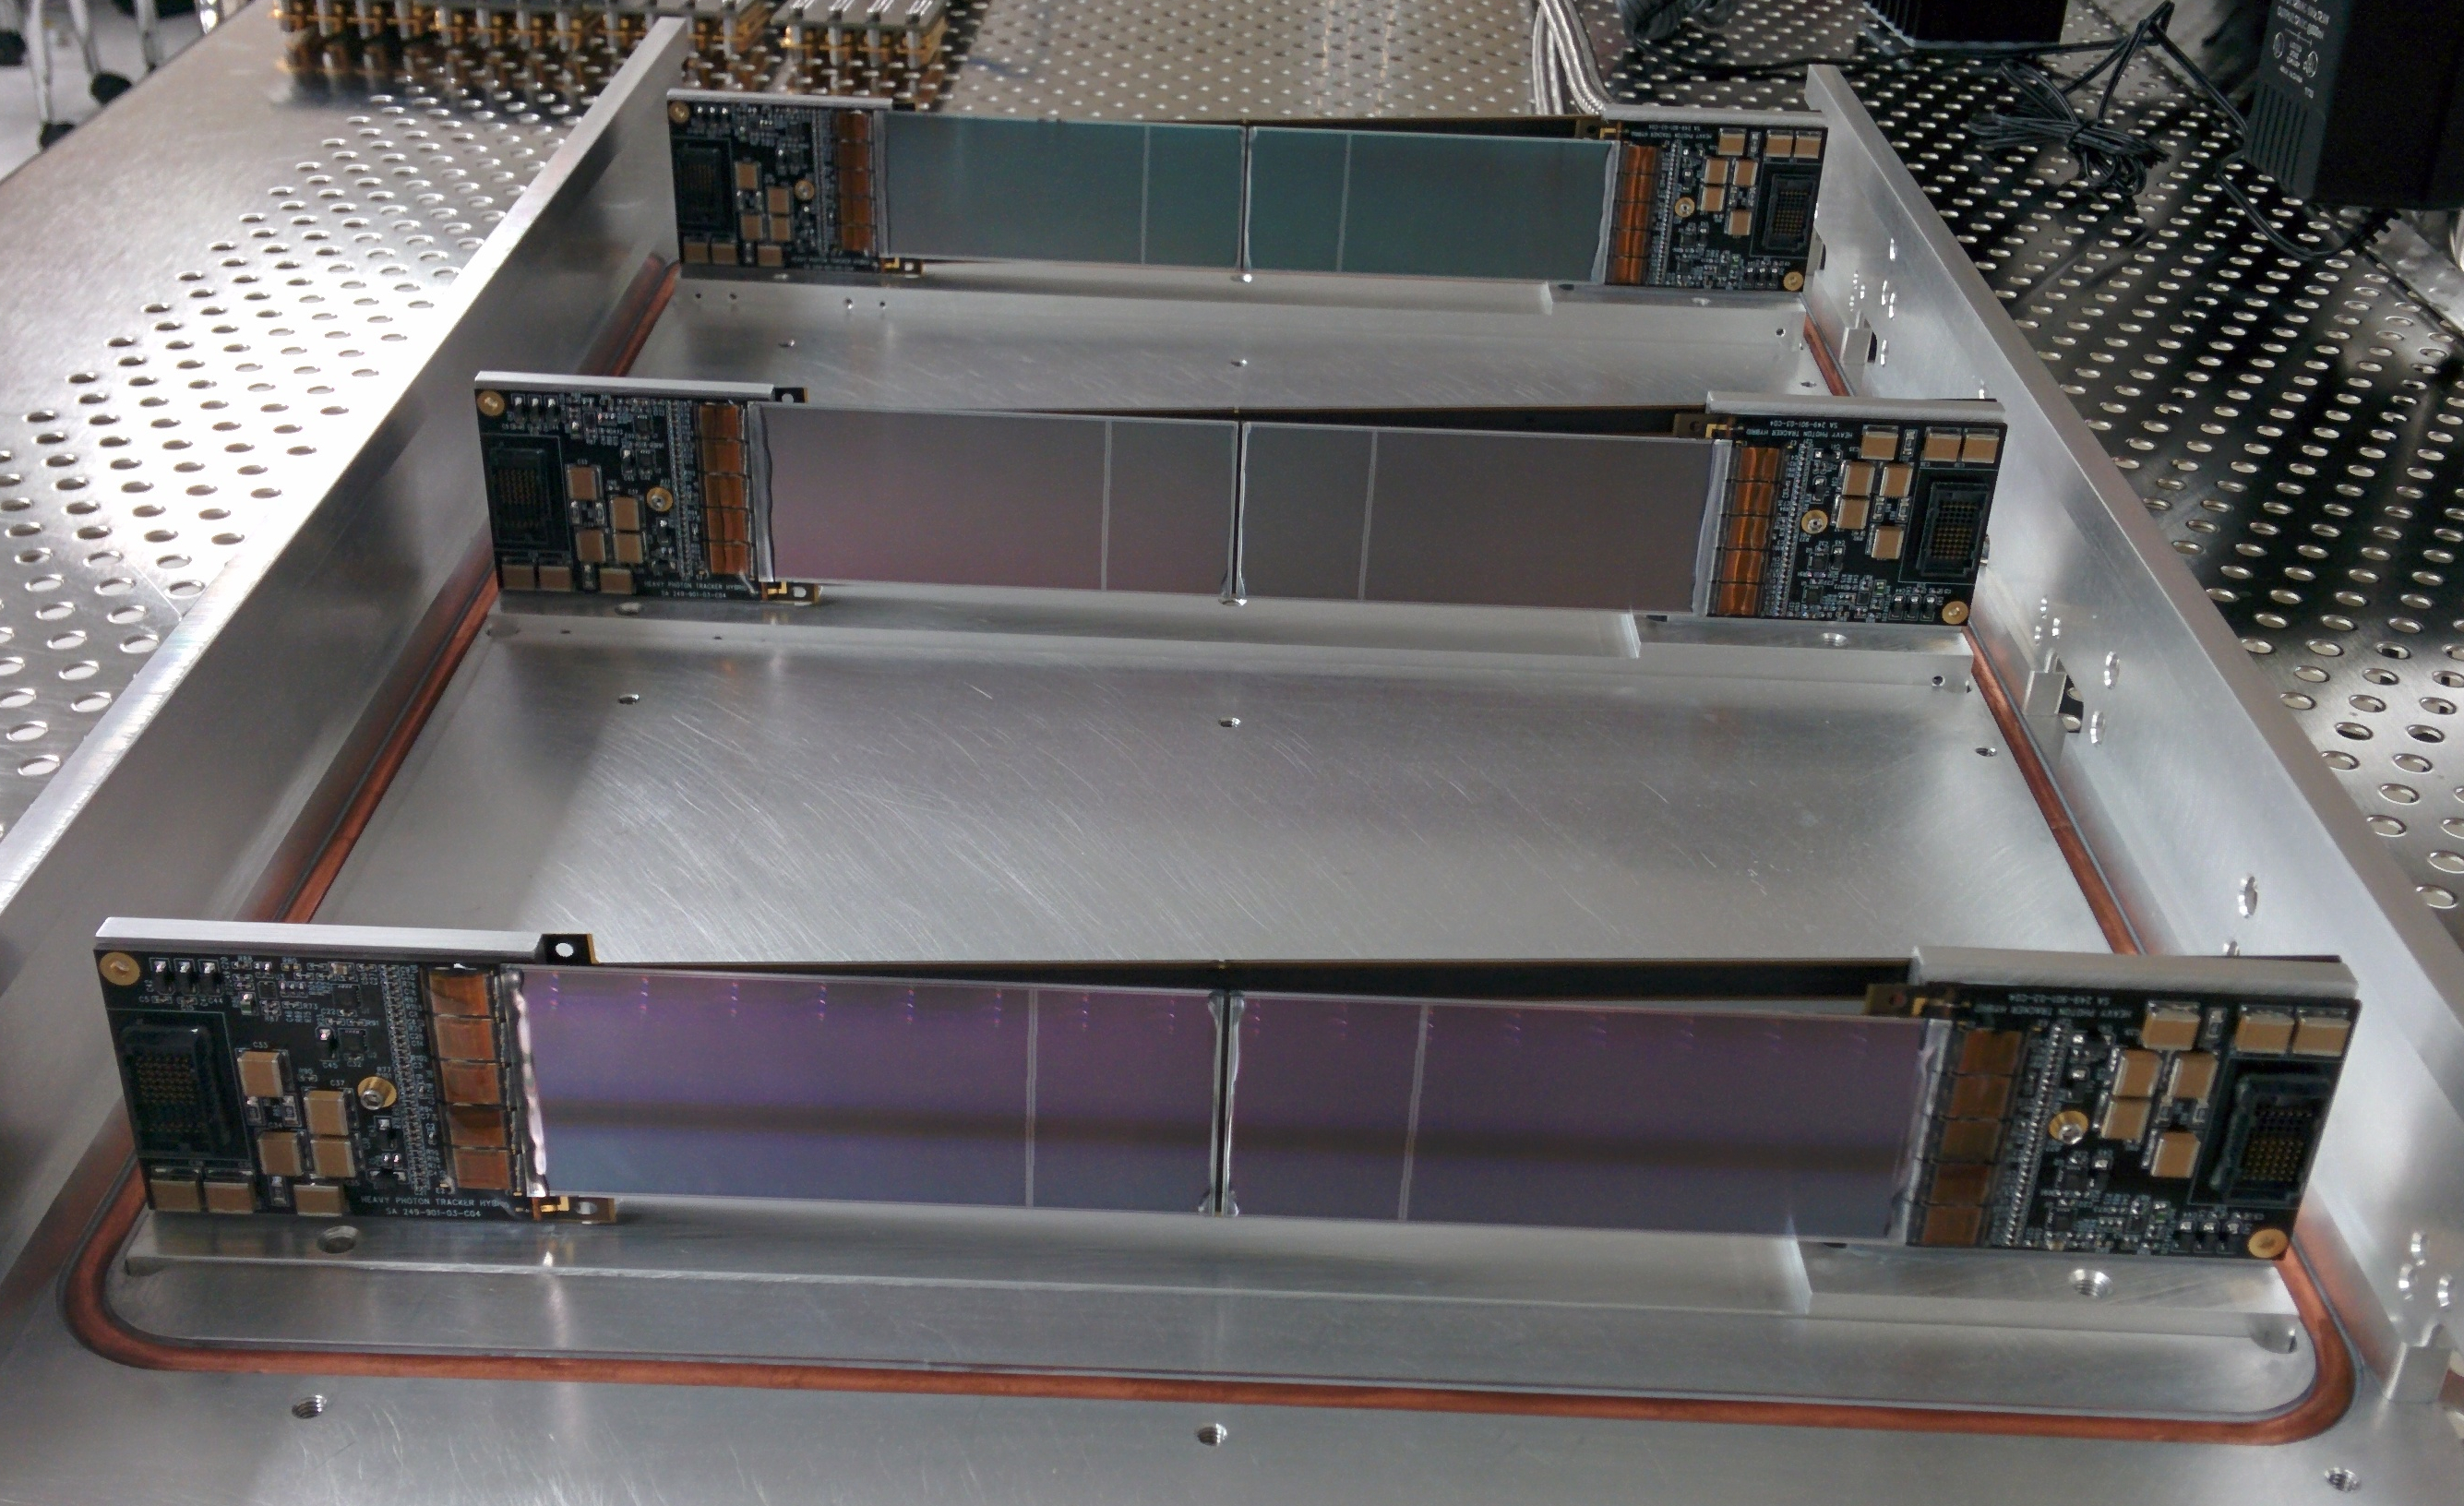
\includegraphics[width=0.9\textwidth]{images/l46_half_module.jpg}
    \caption{A layer 4-6 half-module used by the SVT. }
    \label{fig:l46_hm}
\end{figure}


\subsection{Mechanical Support, Cooling and Services}

...


\section{Electromagnetic Calorimeter}

The HPS Ecal is used as the primary trigger for the experiment as well as to
identify electrons.  It consist of two halves of lead-tungstate 
PbW0$_4$ crystals with each half mounted on an aluminum frame $\sim 137$ cm 
from the upstream edge of the analyzing magnet.  Each half is composed of five
layers of crystals with the four most outer layers consisting of 46 crystals and 
\begin{figure}
    \centering
    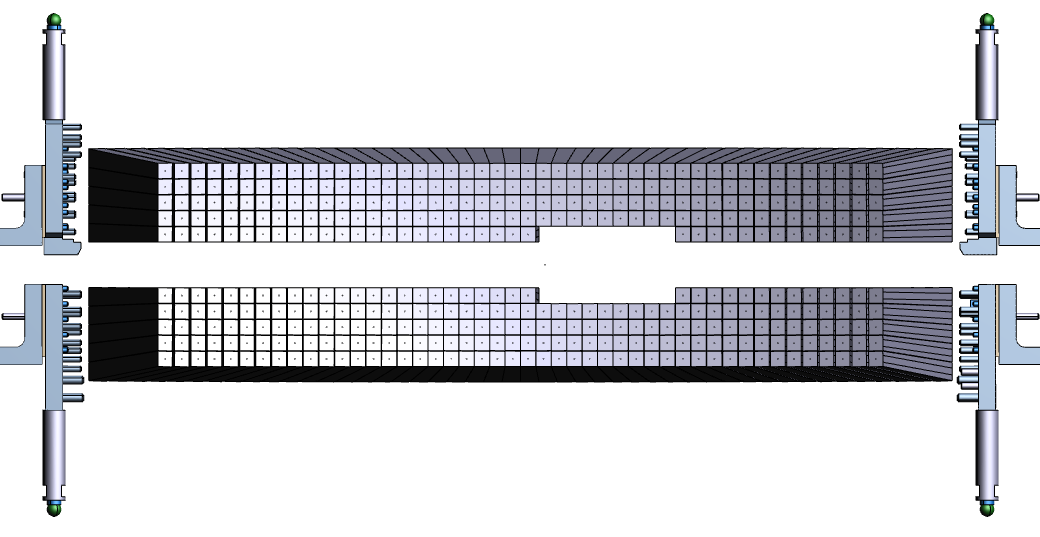
\includegraphics[width=0.8\textwidth]{images/ecal_layout.png}
    \caption{A rendering showing the arrangement of the Ecal crystals.  The Ecal
             is split into upper and lower modules in order to accommodate the 
             ``dead zone''.  The crystals removed from the first layer allow
             a larger opening for the outgoing electron and photon beams.}
    \label{fig:ecal_layout}
\end{figure}
the layer closest to the beam plane consisting of 37. The removal of the 9 
crystals from the inner layer was necessary to allow the outgoing electron and
photon beams to pass through unimpeded.  Each half is enclosed in a temperature
controlled environment held at 1$^{\circ}$ F which encroaches on the Ecal 
vacuum chamber.

Each of the crystals is 16 cm long and trapezoidal in shape with a front face
dimension of $1.3 \times 1.3$ cm$^2$ and a back face dimension of $1.6 \times
1.6$ cm$^2$.  In order to maximize the light yield, the crystals were wrapped
in VM2000 non-metallic reflector film. A Hamamatsu S8664-1010 Avalanche 
Photodiode (APD) with a photosensitive area of $10 \times 10$ mm$^2$ was glued
to the back of each crystal and used to read out the signals collected by the
crystals.  
\begin{figure}
    \centering
    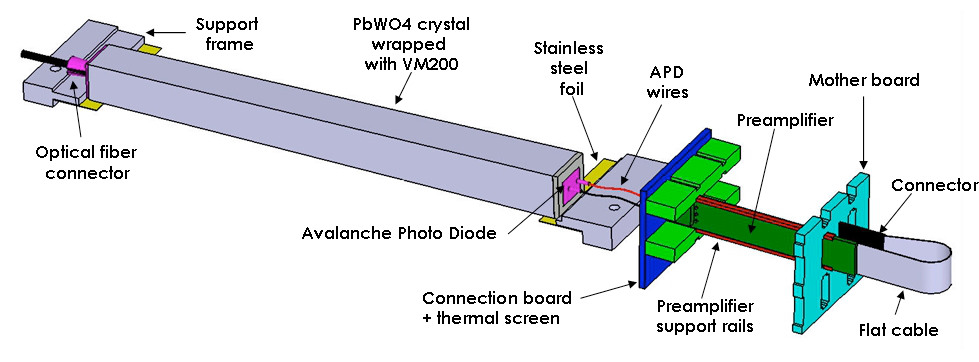
\includegraphics[width=0.8\textwidth]{images/ecal_crystal.png}
    \caption{Rendered view of an HPS Ecal module consisting of a 16 cm PbW$_4$
             crystal, Avalanche Photodiode and preamplifier board.}
    \label{fig:ecal_crystal}
\end{figure}

\section{Trigger and Data Acquisition}

\subsection{Ecal Data Acquisition}

The analog signals that are read out from each of the Ecal crystals by the APDs
are sent a 16-channel JLab FADC250 VXS module (FADC)
(see Figure \ref{fig:ecal_fadc}).  The 221 FADC channels used by each half of 
the Ecal are housed in their own 20 slot VSX crates.
\begin{figure}
    \centering
    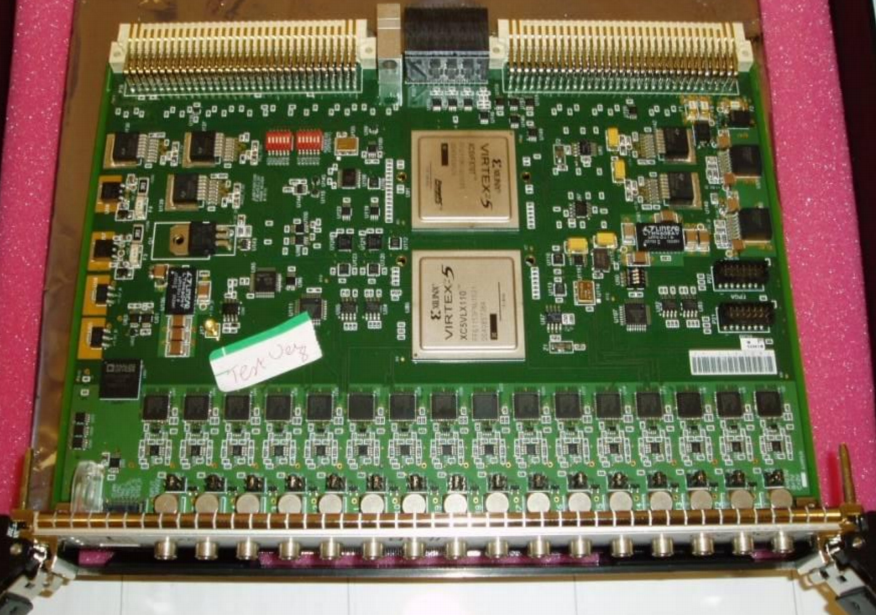
\includegraphics[width=0.7\textwidth]{images/ecal_fadc.png}
    \caption{A 16-channel Jefferson Lab FADC250 VXS module.}
    \label{fig:ecal_fadc}
\end{figure}

The APD signals are sampled and digitized by the FADCs at a rate of 250 MHz
into 8 $\mu$s deep pipelines.  If an FADC signal crosses a pre-defined
threshold, the integrated amplitude of a select number of samples before and
after the threshold crossing, as well as the crossing time are passed to the
Crate Trigger Processor (CTP).

\subsection{Trigger}

The HPS trigger is designed to efficiently select $e^+e^-$ pairs whose energy
depositions, or clusters, in the Ecal are consistent with 
%with either a trident reaction or 
the decay of an $A'$. The trigger logic searches for signals that
are coincident in time and satisfy a specific kinematic selection optimized
to select $A'$ events.

As discussed in the previous section, if a signal from an Ecal crystal is found
to cross some pre-determined threshold, the crossing time and amplitude are 
reported to the CTP. The CTP contains the cluster finding algorithm
which performs the following task: 
\begin{itemize}
    \item The amplitude of hits from every 3x3 array of crystals in the Ecal that
          is within a programmable number of clock cycles is summed. 
    \item If the 3x3 sum exceeds a pre-defined cluster amplitude threshold and
          the sum is greater than any of the neighboring 3x3 windows, then the 
          amplitude (energy), position, time and hit pattern is reported to the Sub-System
          Processor (SSP).
\end{itemize}

The SSP takes the cluster information reported by both halves of the Ecal and
creates all possible pairs of clusters that fall within an 8 ns coincident
window.  Then, in order to further reduce background rates, the following 
selection is applied to the pairs of clusters: 
\begin{itemize}
    \item $E_{min} \le E_{top} + E_{bottom} \le E_{max}$
    \item $| t_{top} - t_{bottom} | \le \Delta t_{max}$
    \item $|E_{top} - E_{bottom} \le \Delta E_{max}$
    \item $E_{low} + R \times  F \le$ Threshold$_{slope}$
    \item $|\tan^{-1}\frac{X_{top}}{Y_{top}} - \tan^{-1}\frac{X_{bottom}}{Y_{bottom}}| \le \theta_{Coplanarity}$
\end{itemize}
Here, $E_{top}$ ($E_{bottom}$), $t_{top}$ ($t_{bottom}$), $x_{top}$ 
($x_{bottom}$) and $y_{top}$ ($y_{bottom}$) are the energy, timestamp and 
position of the cluster in the top (bottom) half of the Ecal and $E_{min}$ 
($E_{max}$) is the minimum (maximum) cluster energy sum. $E_{low}$ is the 
energy of the lowest energy cluster, $R$ is the distance between its 
center and the calorimeter center while $F$ is a constant. As shown on Table
\ref{tab:triggers}, several of these 
parameters are programmable.  The values used during the engineering run are 
listed on Table \ref{tab:triggers}. If a pair of clusters
satisfies these criteria, a trigger signal is generated by the Trigger Supervisor
and sent to all subsystems. 

During the engineering run, several triggers were run simultaneously.  The main
trigger used to select $A'$ type events is the Pair-1 trigger.  The Pair-0 
trigger is a much looser version of the Pair-1 trigger and was tuned to select 
Moller scattering events.  The Single-1 trigger was tuned to select electrons
that Coulomb scatter in the target i.e. full energy electrons (FEE) into the 
acceptance of the Ecal.  These events are used to study both the momentum 
resolution of the tracker and the energy resolution of the Ecal.  Finally, 
there was a cosmic trigger and a pulser trigger used to trigger on cosmic ray
muons and randoms respectively.  A summary of all of the settings is given
on Table \ref{tab:triggers}

\begin{table}
    \centering
    \begin{tabular}{lcccc}
        \toprule
        \textbf{Parameter} & \textbf{Single-0} & \textbf{Single-1} & \textbf{Pair-0} & \textbf{Pair-1} \\
        \midrule
        \midrule
        $E_{min}$ (GeV)      & 0.060 & 0.400 & 0.054 & 0.054 \\
        $E_{high}$ (GeV)     & 2.500 & 1.100 & 1.100 & 0.630 \\
        $N_{threshold}$      & 3     & 3     & 1     & 1     \\
        $E_{sum low}$ (GeV)  &       &       & 0.120 & 0.180 \\
        $E_{sum high}$ (GeV) &       &       & 2.000 & 0.860 \\
        $E_{differenec}$ (GeV) &       &       & 1.000 & 0.540 \\
        $F (GeV)$ & & & 0.0055 \\
        $\theta_{coplanirity}$ & & & 30$^\circ$ \\
        $t_{coplanirity} (ns)$ & & 16 & 12 \\
        Prescale & $2^{13}$ & $2^{11}$ & $2^{10}$ & $2^{0}$ \\
        Rate (50 nA) & 0.4 Hz & 1.3 kHz & 0.7 kHz & 16.6 kHz \\
        \bottomrule
    \end{tabular}
    \caption{The trigger setting for all trigger types used during the 
             engineering run.}
    \label{tab:triggers}
\end{table}



%\subsection{Ecal DAQ}

%\subsection{SVT DAQ}
% Need to discuss the hybrid design for both layers 1-3 and 4-6.
% 1) Need to mention why different wiring was used for the different parts of 
% the SVT.

%After a trigger is received, the differential current signals 
%from each of the APV25's are transferred to a total of 10 Front End Boards (FEB)
%to undergo digitization and further processing. (Add figure?) As discussed in 
%section (), the signals from layers 1-3 are transferred to the FEB's via 
%Teflon-coated twisted pair wires while those emerging from
%layers 4-6 use twisted pair magnet wire.  The use of twisted pairs reduces
%crosstalk between the lines as well as electromagnetic interference.

%At the FEB's, the differential current signals are first converted to a voltage
%by a pre-amplifier circuit to match the dynamic range 
%of the AD9252 14-bit analog to digital converter (ADC). The ADC samples the 
%signal at 41.667 MHz and digitizes it to a value between 0 and 16384.  The 
%digitized signals are then transferred to Xilinx Artix-7 field programmable
%gate arrays (FPGA).  The signals are sent upstream by multi-gigabit transceivers.

%Those signals which pass the threshold requirement are transferred through 
%mini SAS wires to a board on the vacuum  where they undergo optical conversion.
%The optical signal is then transferred over ~10 m fibers to the ATCA crate.


%\subsection{Ecal DAQ}

 % Maybe show an example of how the signal looks emerging from the APV?




%%%%%%%%%%%%%%%%%%%
%   Performance   %
%%%%%%%%%%%%%%%%%%%

\chapter{Detector Performance}

The HPS engineering run took place within Hall B at the Thomas Jefferson 
National Accelerator Facility (JLab) in Newport News, VA in the Spring of 2015.
Although the commissioning of the Ecal had already taken place during a run in 
December of 2014, the engineering run would mark the first time that the SVT 
would take on an electron beam and that both subsystems (SVT, Ecal) would be operating in 
conjunction.  Therefore, the performance results from the engineering run were
critical in verifying that all performance metrics were as simulated and to the
planning of future HPS runs.  In the chapter that follows, a review of a few
selected results that demonstrate the performance of both subsystems during the
engineering run will be given.

\section{Performance of the Silicon Vertex Tracker}

Since it was the first time that the SVT would take on physics quality beam, 
care was taken to understand several performance metrics before continuing to
move the first three layers of the SVT towards their final position. 
%In fact, the SVT was ``timed in'' with layers 1-3 position at 4 mm from the beam plane.  
In fact, data was taken with layers 1-3 of the SVT at several positions above the
beam plane and the occupancies were verified
to match what was expected from simulation.  This was of utmost  
importance since the 1\% occupancy requirement at 0.5 mm was crucial to operation of the
SVT. 

All of the data taken with the SVT saw all APV25s configured to their nominal
operating points as listed in Table \ref{tab:apv_specs}, while all sensors were reverse-biased
to 180 V. All hybrids were being cooled to $\sim$ -14$^{\circ}$C while all FEBs
were being operated at $\sim$ 20$^{\circ}$C.  Finally, only 4 out of the 23,004
SVT channels were found to be dead or noisy.

\subsection{Calibrations}

Preparing the SVT for real physics data-taking required the calibration of the
readout system. This involved the extraction of the baseline 
(pedestal), noise and gain for each of the 23,004 SVT channels.  All 
measurements were made with the APV25s configured to their nominal operating
points and all sensors reverse-biased to 180 V.

The baseline and noise of each of the channels were evaluated by using 
special ``calibration'' runs during which the APV25s were continuously triggered
and read out without any signal present at the input.  The amplitude
of each of the six samples that are 
read out will be Gaussian distributed around the true baseline value with a 
width equal to the noise.  For each of the samples, the baseline distributions
were fit and the baseline and noise extracted (see Figure \ref{fig:baseline_fit}).
\begin{figure}[h!t]
    \centering
    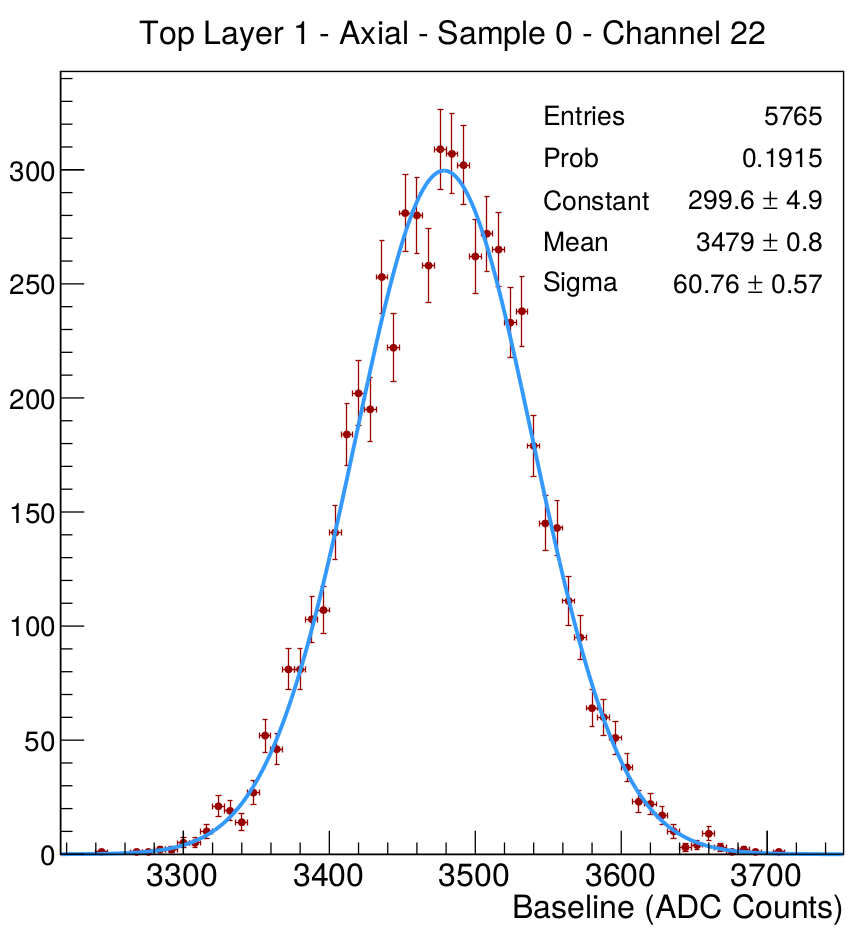
\includegraphics[width=.6\textwidth]{images/baseline_fit_top_l1_axial_sample0_ch22.png}
    \caption{Example illustrating the Gaussian nature of the distribution of
             baseline values.  The distribution is fit with a Gaussian in order 
             to extract the baseline and noise for the channel and sample.}
    \label{fig:baseline_fit}
\end{figure}
A typical distribution of baseline values across a half-module is shown in 
Figure \ref{fig:baseline}.  
\begin{figure}[h!t] 
    \centering
    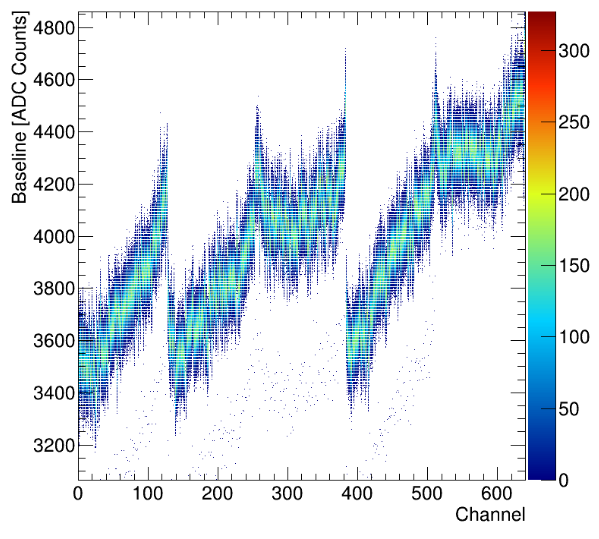
\includegraphics[width=.7\textwidth]{images/baseline.png}
    \caption{Distribution of baseline values across a sensor.}
    \label{fig:baseline}
\end{figure}  
\begin{figure}[h!b]
    \begin{subfigure}{.5\textwidth}
        \centering
        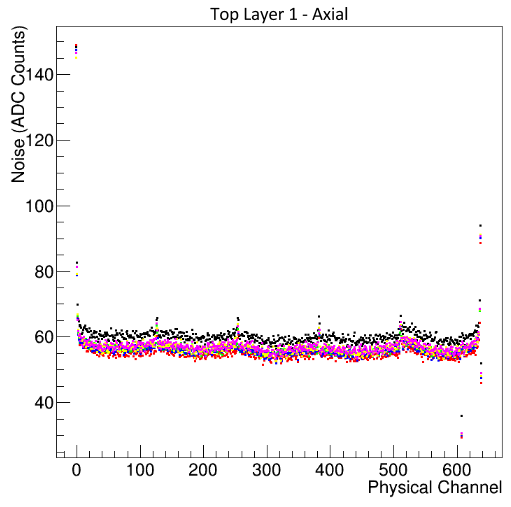
\includegraphics[width=\textwidth]{images/noise_top_layer1_axial.png}
    \end{subfigure}
    \begin{subfigure}{.5\textwidth}
        \centering
        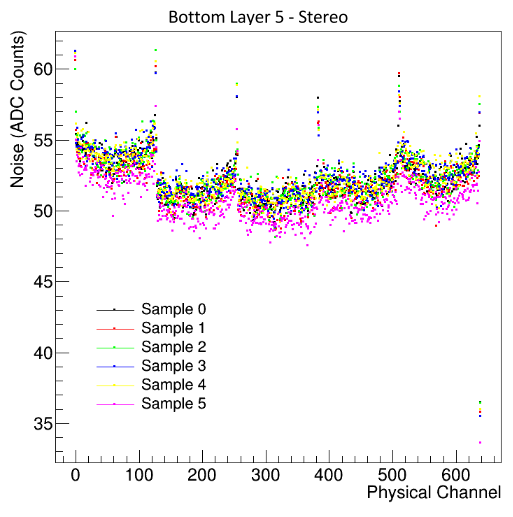
\includegraphics[width=\textwidth]{images/noise_bottom_layer5_stereo.png}
    \end{subfigure}
    \caption{Noise of all channels across a hybrid.}
    \label{fig:noise}
\end{figure}  

Figure \ref{fig:noise} shows the noise across a half-module for each of the 
six samples that are read out.
The noise level of layers 1-3 (4-6) was established
to be between 55-60 (50-55) ADC counts which amounts to $\sim$ 800 - 875 (725 - 800) 
electrons. One thing to note is the large noise values at
the edges of each chip.  This has also been observed by the Compact Muon
Solenoid collaboration
and the cause is still under investigation\footnote{There was an extensive email
discussion with Mark Raymond regarding this issue, but a clear cause was never
pinpointed}. 

The APV25 has a built in calibration circuit that allows for a 
pre-determined signal of known charge to be injected into a subset of channels.
This allows for the accurate determination of the response to a given charge 
via a CR-RC shape fit
to the six pedestal subtracted samples.  The distribution across a hybrid 
of responses to 18,500 electrons is shown in Fig. \ref{fig:response}.
\begin{figure}[h!t]
    \centering
    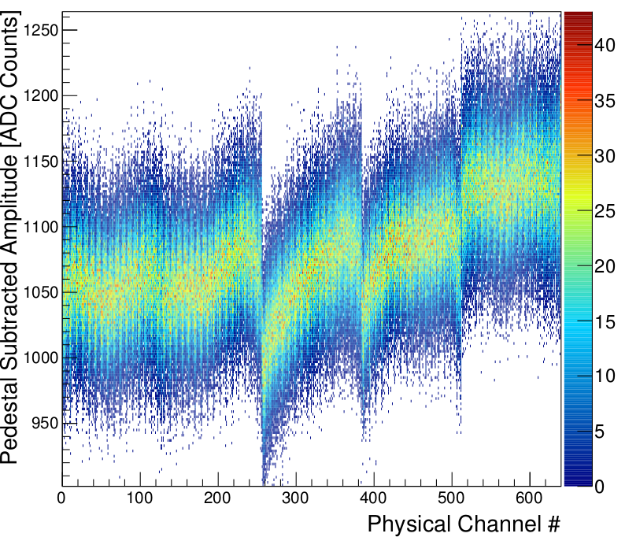
\includegraphics[width=.6\textwidth]{images/response.png}
    \caption{Distribution of responses to 18,500 electrons across one of the 
             half-modules of the Silicon Vertex Tracker.}
    \label{fig:response}
\end{figure}
\begin{figure}[h!b]
    \centering
    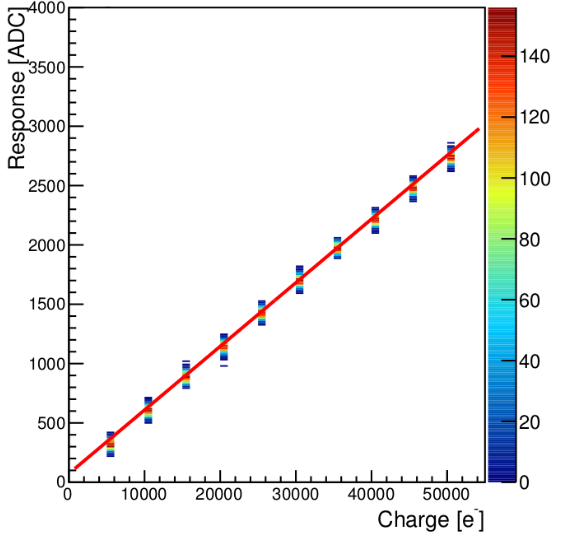
\includegraphics[width=.6\textwidth]{images/response_curve.png}
    \caption{Response curve for a single APV25 channel.}
    \label{fig:response_curve}
\end{figure}
Typically, the response varies by $\sim 7$\% across a half-module. 
The response scale obtained with
the internal calibration circuitry was cross-checked with ionization source
measurements.  

The calibration circuitry was also used to create a response
curve for every channel.  An example of a response curve for one of the 
APV25 channels is shown in Figure \ref{fig:response_curve}.  A linear fit
to the response curve yields the gain and offset of the channel. From the figure, 
it can be seen that the response is approximately linear up to $\sim$ 2 MIPs 
($\sim$ 25,000 $e^{-}$) which is the region of relevance for HPS.
This is in agreement with previous measurements which found the gain to be 
linear up to approximately 3 MIPS \cite{French:2001xb}.

\subsection{Occupancy}

When deciding the extent of the ``dead zone'' between upper and lower portions
of the SVT, aside from avoiding the radiation field, 
two of the main considerations were the ability to perform robust pattern 
recognition and minimization of pileup within the window of time needed for 
the shaper output to evolve ($\sim$ 250 ns for a 50 ns shaping time).  Using
simulation, it was determined that limiting the occupancy of the strips closest
to the beam within an 8 ns window to less than 1\% fulfilled all of the requirements. 

Since the engineering run marked the first time that the SVT had taken an 
electron beam, care was taken when lowering the first three layers to their 
final position a mere 15 mrad from the beam.  In fact, the occupancies 
with layers 1-3 at 4, 3, 2, and 1.5 mm away from the beam plane were verified to
match what was predicted from simulation before the SVT was lowered to its final
position.  As can be seen in Figure \ref{fig:occupancies}, once the first
three layers were lowered into their final position (edge at 0.5 mm away from the
beam plane), the occupancies on the innermost strips were observed to be less
than 1\% as expected.
\begin{figure}[h!b]
    \begin{subfigure}{.5\textwidth}
        \centering
        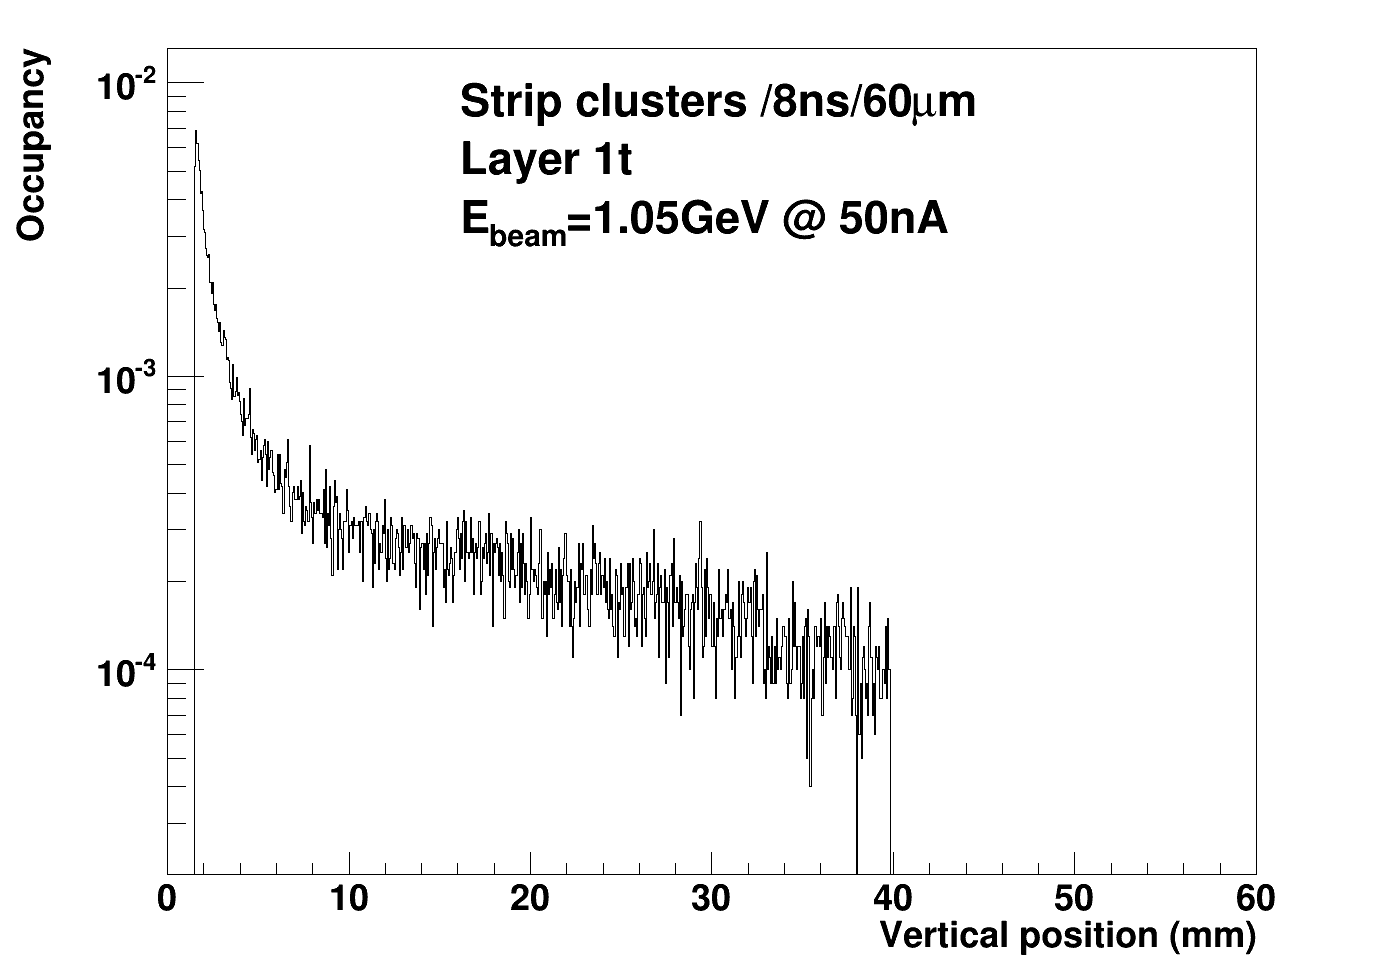
\includegraphics[width=\textwidth]{images/cluster_occupancy_L1t_axial.png}
    \end{subfigure}
    \begin{subfigure}{.5\textwidth}
        \centering
        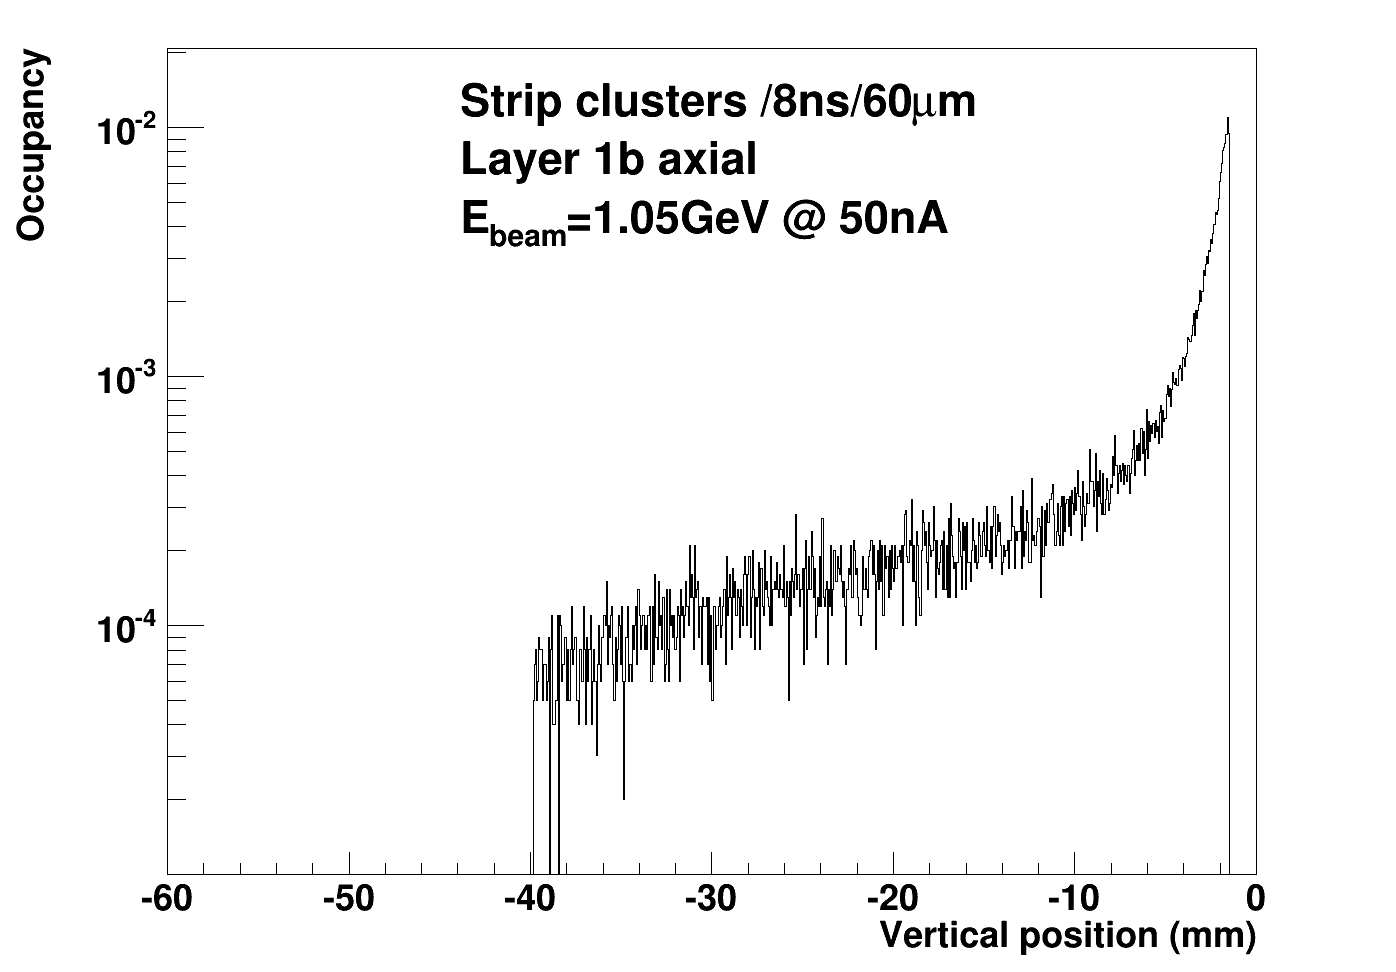
\includegraphics[width=\textwidth]{images/cluster_occupancy_L1b_axial.png}
    \end{subfigure}
    \caption{Occupancies of both top and bottom layer 1.  The occupancies of 
             the innermost strips were observed to be less than 1\% as predicted
             by simulation.}
    \label{fig:occupancies}
\end{figure}  

\subsection{Hit Quality}

When an electron traverses a sensor, the deposited charge may be spread over
several strips.  The signal from each of the strips is processed by the
APV25 and the six samples emerging from each channel are fit using the 
following 3-pole function
\begin{equation}
    f(t) = A\frac{\tau_1^2}{(\tau_1 - \tau_2)^3}\left( e^{-\frac{t-t_{0}}{\tau_1}}
        - \sum_{k=0}^2 \left(\frac{\tau_1 - \tau_2}{\tau_1\tau_2}(t-t_{0})\right)^k
        \frac{e^{-\frac{t-t_{0}}{\tau_2}}}{k!} \right)
\end{equation}
where $\tau_1$ and $\tau_2$ represent the fall and rise time of the shaper 
signal respectively.  The amplitude, $A$, and the time of the hit, $t_0$, are then
determined from the fit.

\begin{figure}[h!t]
    \centering
    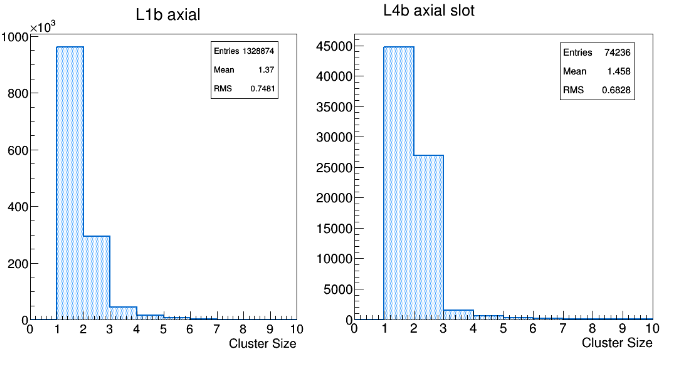
\includegraphics[width=\textwidth]{images/cluster_size.png}
    \caption{The strip multiplicity typically seen during the engineering run.}
    \label{fig:strip_mult}
\end{figure}  
Hits on neighboring strips are clustered using a nearest neighbor
algorithm as follows: 
\begin{itemize}
    \item A list of seeds is created from all raw hits that have an amplitude, $S$,
          $> 4\times \sigma_{\text{Noise}}$
  \item Recursively add neighboring strips that have a $S> 3 \times \sigma_{\text{Noise}}$
          until a strip with $S < 3\times \sigma_{\text{Noise}}$ is found.
      \item Require that neighboring hits have a $t_{0}$ that is within 8 ns of the seed hit.
    \item Repeat the first two steps until seed strips are no longer found.
\item Require that a cluster has an amplitude $> 4 \times \sigma_{\text{Noise}}$.
\end{itemize}
The typical strip multiplicity observed during the run is shown in Figure 
\ref{fig:strip_mult}. Figure \ref{fig:cluster_charge} shows the characteristic
\begin{figure}[h!t]
    \centering
    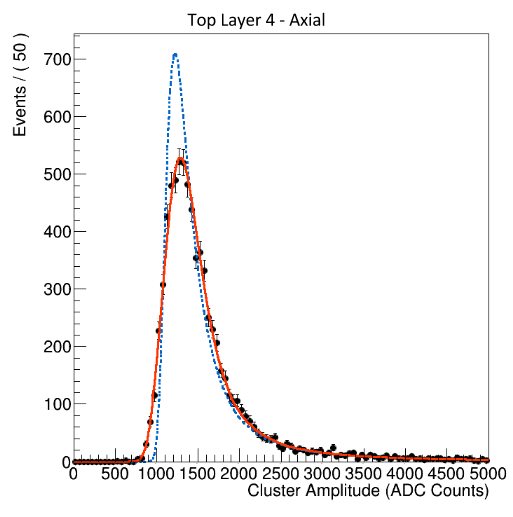
\includegraphics[width=.7\textwidth]{images/top_layer4_axial_cluster_charge.png}
    \caption{Distribution of cluster charge exhibiting the characteristic Landau
    shape.  The cluster charge was fit with a Landau (dashed blue line) convoluted
with a Gaussian (convolution shown in red) in order to extract the most probable value.}
    \label{fig:cluster_charge}
\end{figure}  
Landau shape of the cluster charge distribution for one of the sensors.
The cluster charge distributions of every layer were fit using a Landau
convoluted with a Gaussian in order to extract the most probable value.  The 
cluster charge for all layers were measured to be between $\sim$1400-1500 ADC counts
which corresponds to $\sim$21,000-22,500 $e^{-}$.  

Measuring the signal-to-noise of a sensor was done by simply taking the 
cluster charge amplitude for all single strip clusters and dividing it by
the noise of the channels.  Using this procedure, 
the signal-to-noise of all layers was measured to be within $\sim$24-26, 
as expected (See Figure \ref{fig:sig_noise}).
\begin{figure}[h!t]
    \centering
    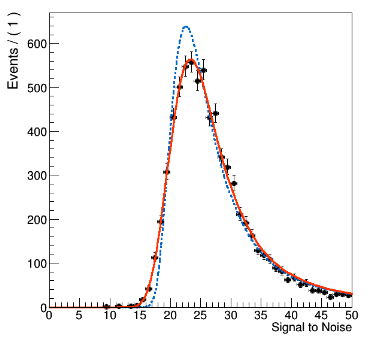
\includegraphics[width=.7\textwidth]{images/sig_noise.png}
    \caption{Example of signal to noise measured during the engineering run.
             The signal-to-noise was fit with a Landau (dashed blue line) 
             convoluted with a Gaussian (convolution shown in red)
             in order to extract the most probable 
             value.}
    \label{fig:sig_noise}
\end{figure}  

After hits on a sensor have been
clustered, the cluster time is computed as the amplitude-weighted average
of the $t_0$ times from the hits that compose it.  In order to study the hit
time resolution, first a ``track time'' is computed by averaging the cluster 
times of all clusters composing a track.  Then, the residual of each of the 
cluster times is
calculated and the resulting distribution per layer is fit with a Gaussian
to extract the $t_0$ resolution.  The resulting distribution and fit for 
one of the layers in the SVT is shown in Figure \ref{fig:t0_res}.  
\begin{figure}[h!b]
    \centering
    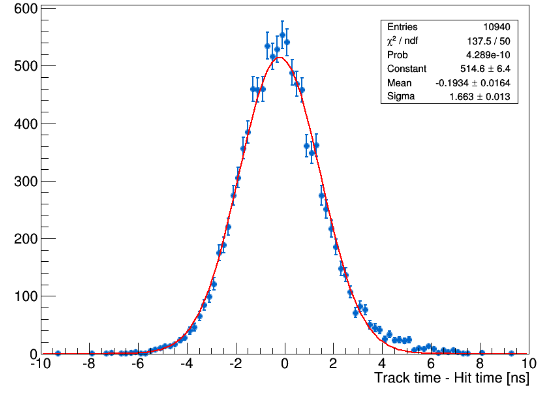
\includegraphics[width=.7\textwidth]{images/t0_res.png}
    \caption{Distribution of cluster time residuals for a single layer of
    the SVT.}
    \label{fig:t0_res}
\end{figure} 
After correcting for offsets and the correlation between hit times, 
the $t_{0}$ resolution is observed to be $\sim$ 
1.8 ns.

\subsection{Momentum Resolution}

Beam electrons that multiple Coulomb scatter in the target can be used  
not only to verify that the momentum scale is correct but also determine the 
momentum resolution.  These full energy electrons (FEEs) 
were selected by requiring a cluster in the Ecal to have a matching track and
to satisfy the following criteria:
\begin{itemize}
    \item The energy of the cluster of interest in the Ecal  is between 0.8 GeV
          and 1.1 GeV.
    \item The time of the cluster seed relative to the trigger time is between
          39.5 ns and 49.5 ns.
    \item The number of hits composing the cluster has to be greater than 3.
    \item The energy of the cluster seed has to be greater than 400 MeV.
    \item Only consider clusters whose position is above the first row of the 
          Ecal.
\end{itemize}
The momentum distributions of the tracks matched to the clusters that pass the
criteria are shown in Figures \ref{fig:top_p} and \ref{fig:bot_p}, split up by volume.  The peaks
of both distributions show that the momentum scale is accurate to within 1\% 
which is an indication that the detector is well aligned.  The 
multiple scattering limited momentum resolution of the top (bottom) was measured
to be $\sigma_{p}/p = 6.8\%$ ($\sigma_{p}/p = 7.1\%$) which 
is within 5\% of of the expected value.
\begin{figure}[h!t]
    \centering
    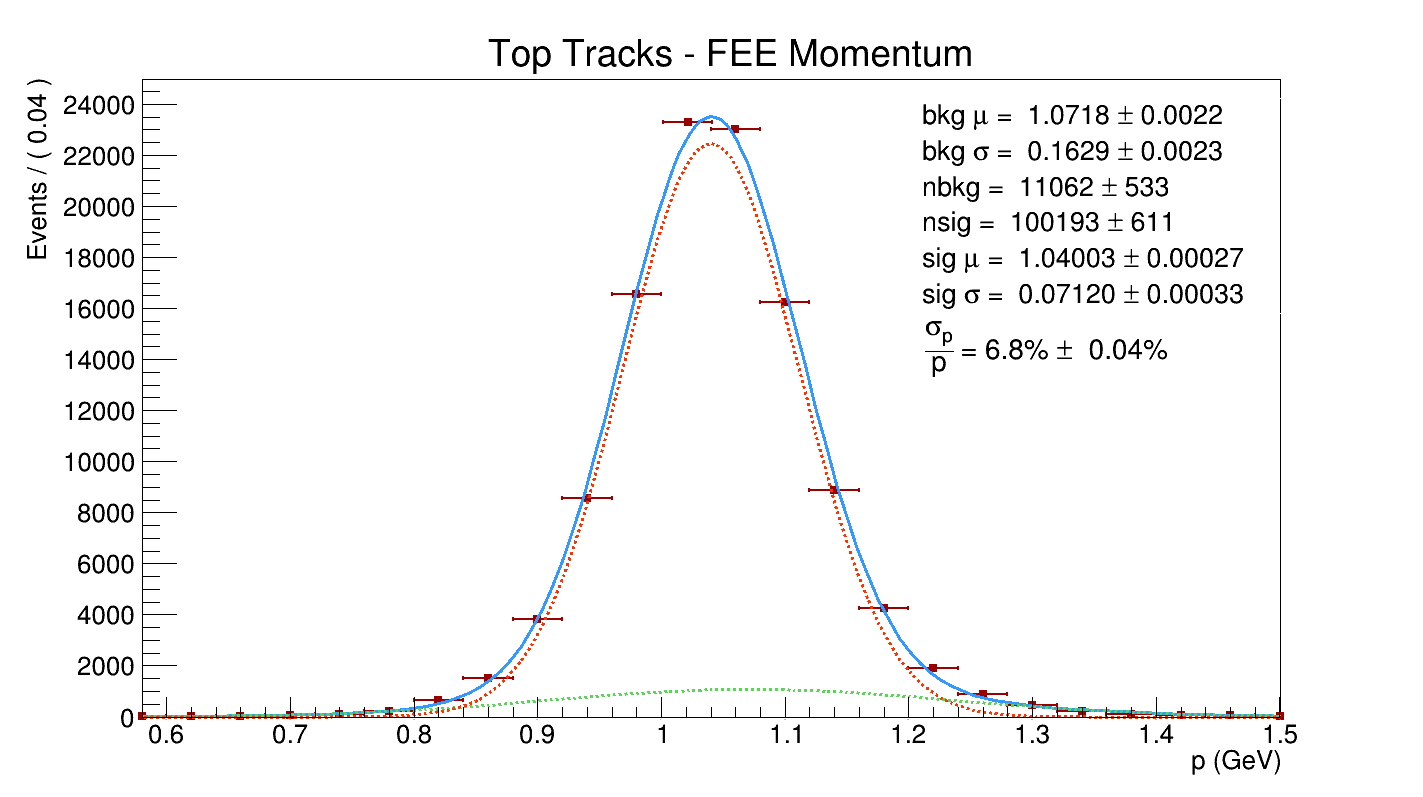
\includegraphics[width=.95\textwidth]{images/20160424_fee_top_tracks_p.png}
    \caption{Mometum distribution of multiple Coulomb scattered electrons (FEE) in
             the top portion of the SVT and Ecal. 
             The mean of the distribution 
             is within $\sim$1\% of the beam energy (1.056 GeV), indicating that 
             the detector is well aligned.}
    \label{fig:top_p}
\end{figure}
\begin{figure}[h!b]
    \centering
    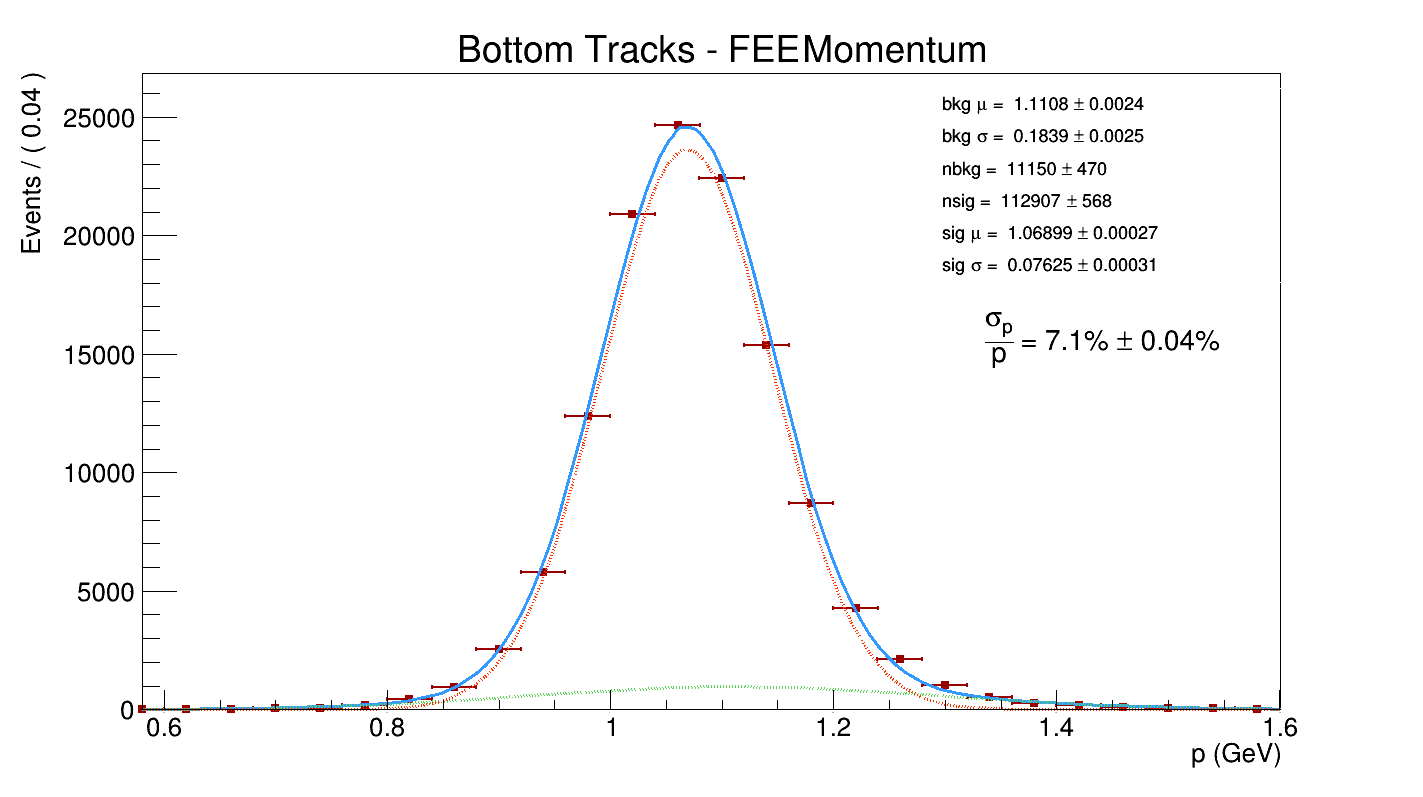
\includegraphics[width=.95\textwidth]{images/20160424_fee_bottom_tracks_p.png}
    \caption{Mometum distribution of multiple Coulomb scattered electrons (FEE) in
             the bottom portion of the SVT and Ecal.
             The mean of the distribution 
             is within $\sim$1\% of the beam energy (1.056 GeV), indicating that 
             the detector is well aligned.}
    \label{fig:bot_p}
\end{figure}

\subsection{Tracking Efficiency}

The electron efficiency was calculated using a tag-and-probe technique.  First
two clusters that are coincident in time are selected in the calorimeter. One
cluster must be on the positron side, i.e. $x > 0$, and the other on the electron
side.  The sum of the momentum of the two clusters in required to be greater 
than 0.8 GeV since this is the region of interest for analysis purposes. Then, 
the positron side cluster is required to match to a positron track.  This 
becomes the tag.  The cluster on the electron side is then checked a 
match to an electron track.  The electron efficiency is then calculated as 
\begin{equation}
    \varepsilon = \frac{N_{probes}}{N_{tags}}.
\end{equation}
Using this method, the electron efficiency was found to be $\sim$ 95\%. A similar
procedure was used to find the positron efficiency to be $\sim$ 95\%.

\subsection{Mass resolution} \label{sec:mass_res}

The heavy photon signal is expected to appear as a Gaussian peak above the QED 
trident invariant mass spectrum with the width corresponding to the mass 
resolution of the experiment.  Thus, determining the mass resolution is a crucial
component of the resonance search, the details of which will be given in Chapter 6.

Parameterizing the mass resolution from data was accomplished by using electron-electron
elastic scattering (M\o ller scattering) which will have a well defined mass.
For this particular study, only events which satisfy the ``singles1'' trigger 
requirements were used.  Furthermore, only events where the bias of the SVT was 
on, the SVT was positioned at 0.5 mm from the beam plane and were free of 
data acquisition errors were considered.

Selection of M\o ller events begins with the requirement that an event have a
pair of clusters in the Ecal coincident in time satisfying the following criteria:
\begin{itemize}
    \item The two clusters must be coincident within a 1.6 ns window.
    \item The two clusters must be in opposite detector volumes.
    \item The $x$ position of both clusters must be $<0$, i.e. both clusters
          are on the electron side.
\end{itemize}
Once a pair of candidate clusters is found, they are required to match to 
$e^-$ tracks.  Both the tracks are then subjected to the following criteria:
\begin{itemize}
    \item Both tracks are subjected to a $\chi^{2}$ probability cut of 95\%.
    \item The momentum of the tracks are required to be less than 0.7 GeV.
    \item The two electron tracks must come from the same vertex.  In order to
          ensure this, the vertex $\chi^2 <$ 10. The positions along $x$ and $y$
          are then required to lie within an ellipse defined as
          \[
                v_x^2/0.04 + v_y^2/0.0025  = 1.
          \]
\end{itemize}
Finally, the momentum sum of the tracks associated with the clusters must be
greater than 0.8*1.056 GeV and less 1.2 GeV.  The resulting M\o ller distribution
is shown in Figure \ref{fig:moller_mass}. 

In order to extract the mass resolution, the invariant mass distribution was 
fit with a Crystal Ball function \cite{Gaiser:1982yw} given by 
%\begin{equation}
%    f(x; \alpha
%    \begin{cases}
%
%    \end{cases}
%\end{equation}
plus a Gaussian to account for accidental 
$e^-e^-$ on the low side (See Figure \ref{fig:moller_mass}).  From the 
fit, the mass peak is found to be at 33.2 MeV which is within 3\% of the design
value.  The mass resolution at 33.2 MeV is 1.4 MeV which is within 10\% of what
was predicted by simulation.
\begin{figure}[h!t]
    \centering
    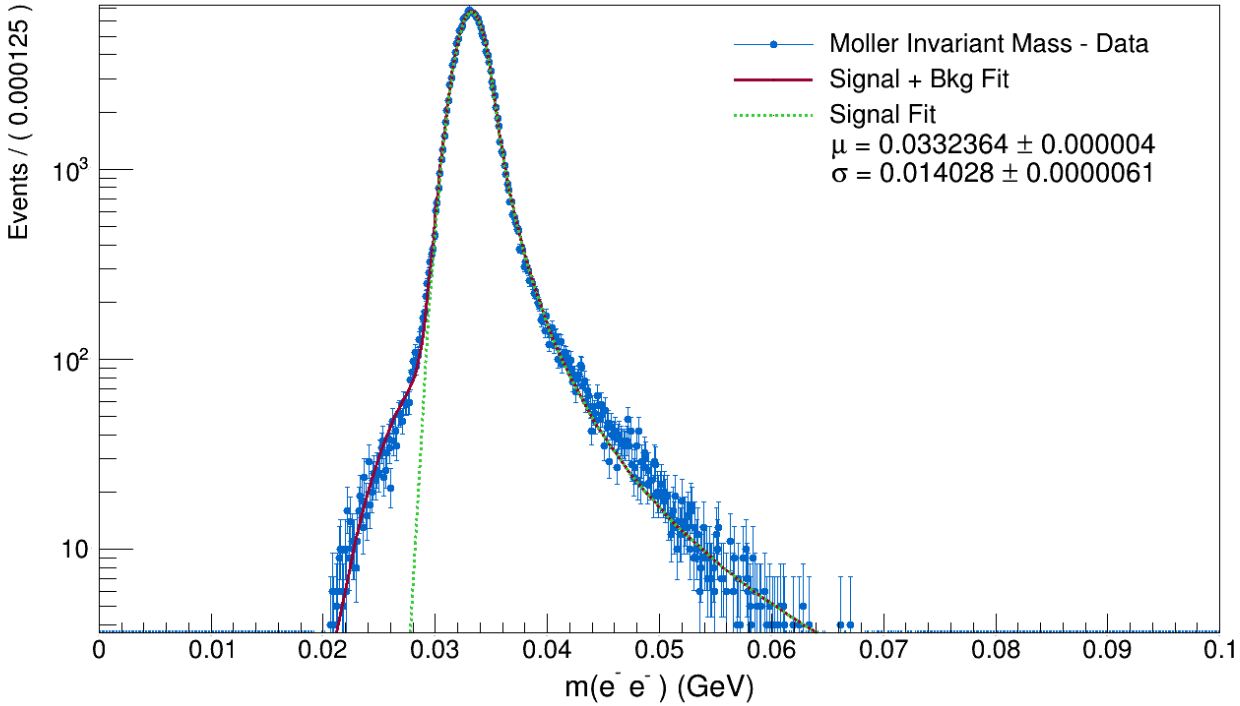
\includegraphics[width=\textwidth]{images/moller_invariant_mass.png}
    \caption{M\o ller invariant mass distribution.}
    \label{fig:moller_mass}
\end{figure}

Determining the mass resolution as a function of mass was done by using $A'$ 
signal and M\o ller Monte Carlo. The resulting mass resolutions at each mass 
hypothesis are shown in Figure \ref{fig:mass_resolution}. 
\begin{figure}[h!t]
    \centering
    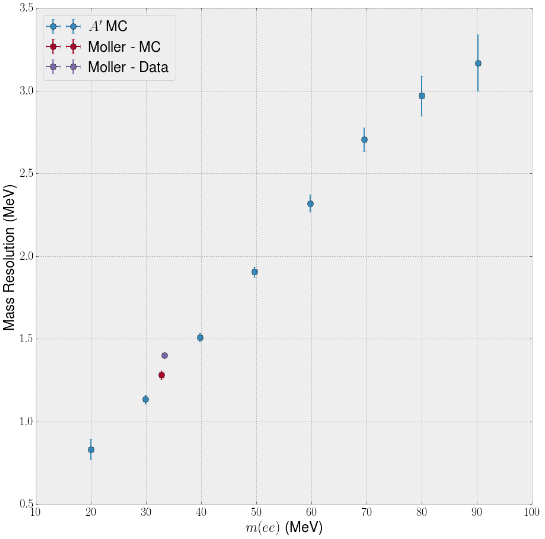
\includegraphics[width=.8\textwidth]{images/invariant_mass_curve.png}
    \caption{The mass resolution as a function of mass calculated using 
              the invariant mass distributions of
              $A'$ (blue) and M\o ller Monte Carlo (red) as well as M\o ller 
         data (purple).  The mass resolution calcualted using data is within
            10\% of the expected value calculated with Monte Carlo.}
    \label{fig:mass_resolution}
\end{figure}
The mass resolution as a function of mass was found to be best modeled using
a third order polynomial of the form
\begin{equation}
    \sigma_{m}(m_{ee}) = -6.166 m_{ee}^3 + 0.9069 m_{ee}^2 - 0.00297 m_{ee} + 0.000579 \text{ GeV}
\end{equation}
This equation was used in the resonance search described in Chapter 5. 

\section{Performance of the Electromagnetic Calorimeter}

Beam electrons that multiple Coulomb scatter in the target can also be used to 
determine the energy resolution of the calorimeter.  The resulting resolution 
measured in this manner was determined to be $\sim$ 4\% and is shown in Figure
\ref{fig:energy_res}.
\begin{figure}[h!t]
    \centering
    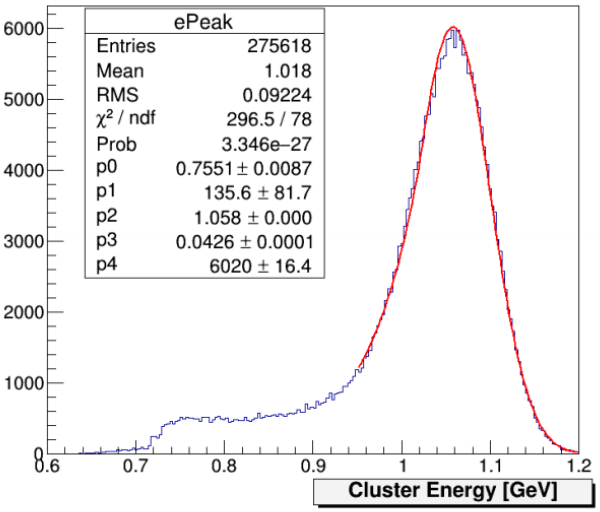
\includegraphics[width=.7\textwidth]{images/ecal_energy_resolution.png}
    \caption{Energy distribution of multiple Coulomb scattered electrons in the
             in the Ecal.}
    \label{fig:energy_res}
\end{figure} 

\section{Trigger Performance}

The performance of the trigger was studied by using a simulation of the trigger
and comparing it to the hardware trigger.  First, the raw FADC hits are converted
to simulated clusters using a simulation of the hardware clustering algorithm. Then
a simulation of the trigger decision was compared to the actual decision reported
by the hardware trigger.  The efficiency is calculated as 
\begin{equation}
\epsilon = \frac{N_{\text{trigger, hardware}}}{N_{\text{trigger, simulated}}}
\end{equation}
The results of the study are listed in Table 
\ref{tab:trig_eff}.
\begin{table}[h!]
    \centering
    \begin{tabular}{lc}
        \toprule
        \textbf{Trigger Type} & \textbf{Efficiency} \\
        \midrule
        \midrule
        Singles               & 99.6\%              \\
        Pair                  & 99.7\%              \\
        \bottomrule
    \end{tabular}
    \caption{Trigger efficiency of both Singles and Pair triggers.}
    \label{tab:trig_eff}
\end{table}





%%%%%%%%%%%%%%%%%%%%%%%
%   Event Selection   %
%%%%%%%%%%%%%%%%%%%%%%%
%
%
%
%
\chapter{Event Selection}

Searching for a heavy photon resonance requires both the accurate 
reconstruction of the QED trident invariant mass spectrum and the efficient 
rejection of Bethe-Heitler events.  With this in mind, a scheme 
was developed to select events with $e^+e^-$ pairs whose kinematic signatures
resemble that of QED tridents which, in turn, mirror the kinematics of 
heavy photon production and decay.  Once a sample of QED tridents has been selected, 
additional kinematic 
requirements were applied to reject Bethe-Heitler events.  The  $e^+e^-$ events
which satisfied all criteria were used to produce the final invariant mass 
spectrum employed to search for a heavy photon resonance.  The following chapter
will discuss the selection used to arrive at the final event sample.   

\section{Data}

The data used for this analysis consist of the unblinded portion of the 2015 
HPS engineering run.  This amounts to approximately $\sim$10\% of the total 
data collected during the run.  The list of runs used in this analysis along
with the unblinded number of events and luminosity for each run 
are shown on Table \ref{tab:data}.
%%%%%%%%%%%%%%%%%%%%%
%   Table of Data   %
%%%%%%%%%%%%%%%%%%%%%
\begin{table}[t]
    \centering
    \begin{tabular}{ccc}
        \toprule
        \textbf{Run Number} & \textbf{Total Events (M)} & \textbf{Luminosity (nb$^{-1}$)} \\
        \midrule
        \midrule
        5723 & 10.68765  & 3.927681901  \\
        5724 & 11.397637 & 4.229082832    \\
        5725 & 8.612363  & 3.193363425   \\
        5739 & 8.0932    & 2.956111602   \\
        5741 & 10.97741  & 3.987840806   \\
        5742 & 11.174619 & 4.224543485   \\
        5743 & 6.040229  & 2.244021498 \\
        5766 & 9.927829  & 3.337962213 \\
        5769 & 11.179994 & 4.059284573 \\
        5771 & 11.642768 & 4.254619178 \\
        5772 & 11.865312 & 4.403638304 \\
        5773 & 13.429284 & 5.014898695 \\
        5775 & 5.580172  & 1.988647799 \\
        5776 & 8.121968  & 2.997741852 \\
        5782 & 12.396243 & 4.552604162 \\
        5783 & 12.226626 & 4.548117122 \\
        5791 & 10.58427  & 3.716081116 \\
        5795 & 8.789774  & 3.17431154 \\
        5796 & 12.055927 & 4.323879491 \\
        5797 & 10.047503 & 3.584285692 \\ 
        \bottomrule
    \end{tabular}
    \caption{List of ``golden'' runs from the 2015 Heavy Photon Search Engineering Run used
             in this analysis along with the total number of events
             and luminosity of the unblinded portion of the data.}
    \label{tab:data}
\end{table}

\section{Event Selection}

The HPS ``pairs1'' trigger was designed to trigger on events with two clusters
whose positions in the Ecal were consistent with an $e^+e^-$ from either a trident 
reaction or the decay of an $A'$. As such, only ``pairs1'' trigger events
were considered for the final data sample.  Furthermore, only events where the
bias of the SVT was on, the SVT was positioned at 0.5 mm from the beam and 
were free of data acquisition errors were included in the data sample.

\subsection{Cluster Pair Selection}

The acceptance of the HPS detector is optimized such that the $e^+e^-$ pairs
produced in either a QED trident reaction or from the decay of an 
$A'$ are observed through their energy depositions in the Ecal.  The energy
depositions or clusters are expected to be in opposite Ecal volumes i.e. 
top/bottom and coincident in time within a coincidence window of a few ns.  This
can be seen from Fig. \ref{fig:cluster_times_2d}, which plots the time relative to 
the trigger time (cluster time) of one cluster composing a pair versus the 
other.  From the figure, it can be seen that most cluster pairs of interest are 
%%%%%%%%%%%%%%
%   Figure   %
%%%%%%%%%%%%%%
\begin{figure}[t]
    \centering
    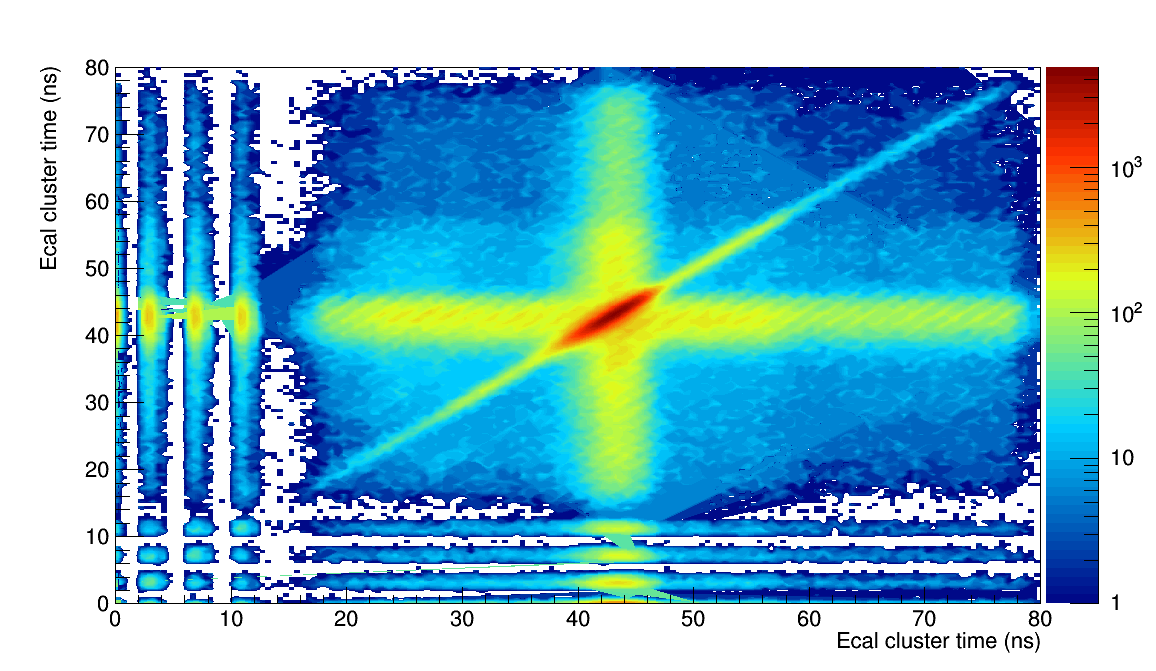
\includegraphics[width=.9\textwidth]{images/20160428_pass4_cluster_time_v_cluster_time.png}
    \caption{The spectrum of Ecal cluster times of one cluster composing a pair 
             versus other.  The figure clearly shows that most coincident pairs 
             fall within tight coincidence and cluster time windows.}
    \label{fig:cluster_times_2d}
\end{figure}  
%%%%%%%%%%%%%%
%   Figure   %
%%%%%%%%%%%%%%
coincidence to within a few ns. Furthermore,  
%%%%%%%%%%%%%%
%   Figure   %
%%%%%%%%%%%%%%
\begin{figure}[t]
    \centering
    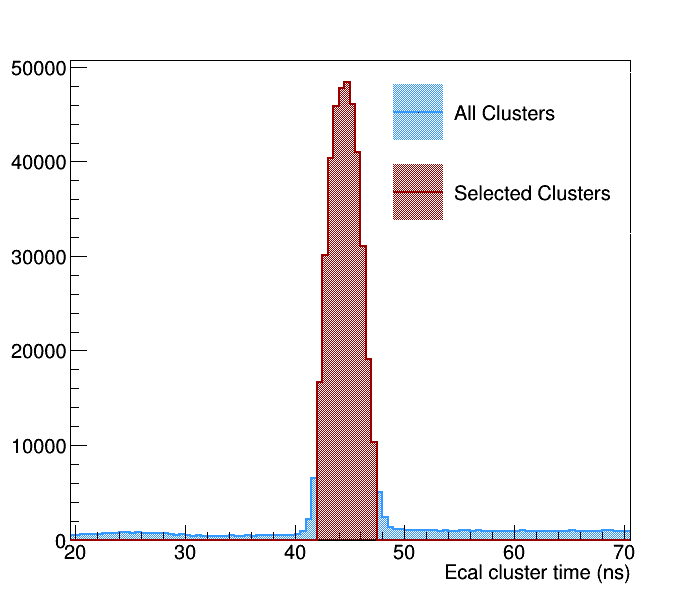
\includegraphics[width=.9\textwidth]{images/20160428_ecal_cluster_time.png}
    \caption{The time relative to the trigger time of all Ecal clusters.}
    \label{fig:cluster_times}
\end{figure}  
%%%%%%%%%%%%%%
%   Figure   %
%%%%%%%%%%%%%%
all clusters also fall within a cluster time window (see Fig. \ref{fig:cluster_times}). 

In order to select true coincidences, the clusters forming a pair were 
required to have a cluster time between 42 ns and 47.5 ns.  The efficiency
of finding a track associated with a cluster was found to dramatically drop 
for clusters outside of this window.  The selection is
shown graphically in red on Fig. \ref{fig:cluster_times}.  Clusters satisfying
the cluster time criteria are then formed into pairs.  The coincidence timing
between a pair is then required to fall within a 3.2 ns window around the 
coincidence peak located at 0.003 ns (Fig. \ref{fig:coin_time}).  If an event
contains multiple ``good'' cluster pairs, the pair with the smallest coincident
time is chosen. 
%%%%%%%%%%%%%%
%   Figure   %
%%%%%%%%%%%%%%
\begin{figure}[t]
    \centering
    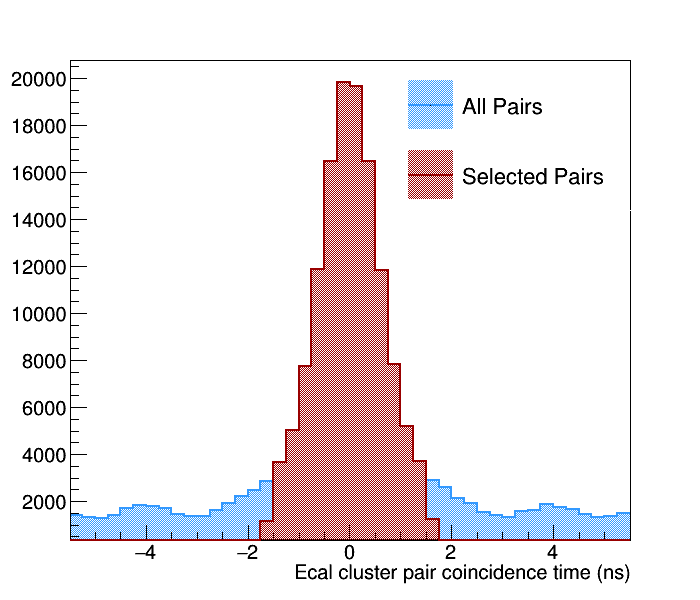
\includegraphics[width=.9\textwidth]{images/20160428_coincidence_time.png}
    \caption{Coincidence time between two clusters in an event.}
    \label{fig:coin_time}
\end{figure}  
%%%%%%%%%%%%%%
%   Figure   %
%%%%%%%%%%%%%%
 
\subsection{Track-Cluster Matching}
   
In order to further suppress accidentals due to one or both clusters in the pair
being attributed to a photon, the 
selected ``good'' cluster pairs are required to have tracks associated 
with them. The trajectories of all tracks in an event are propagated downstream
to the face of the Ecal using the full 3D magnetic field map.  A track and a cluster
are considered a match if the difference between their positions in both $x$ 
and $y$ satisfy the criteria listed on Table \ref{tab:track_cluster_cuts}. The 
cuts were chosen such that they create a 3$\sigma$ window around the peak of 
the cluster-track position difference distributions. The resulting selection is 
highlighted in red on 
Figs. \ref{fig:track_cluster_delta_x} and \ref{fig:track_cluster_delta_y}.
\begin{figure}[h]
    \begin{subfigure}{.5\textwidth}
        \centering
        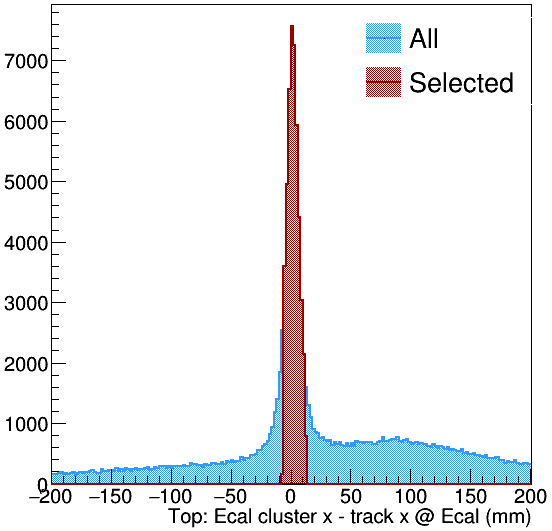
\includegraphics[width=0.85\textwidth]{images/20160502_pass4_cluster_track_delta_x_top.png}
    \end{subfigure}
    \begin{subfigure}{.5\textwidth}
        \centering
        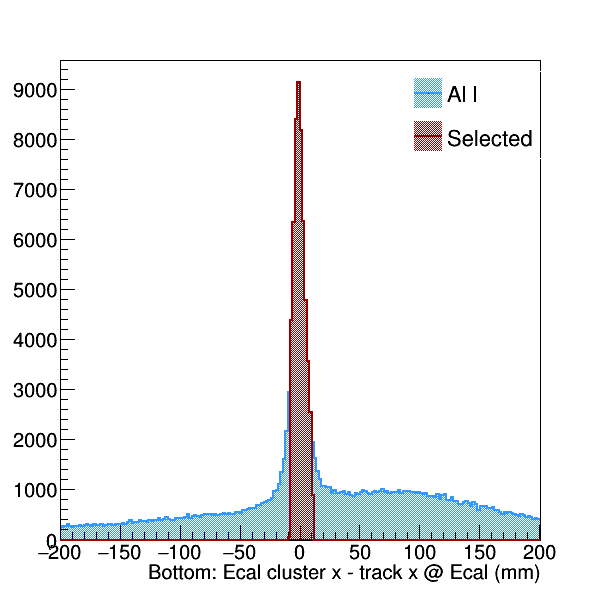
\includegraphics[width=0.85\textwidth]{images/20160502_pass4_cluster_track_delta_x.png}
    \end{subfigure}
    \caption{Histogram}
    \label{fig:track_cluster_delta_x}
\end{figure}
\begin{figure}[h]
    \begin{subfigure}{.5\textwidth}
        \centering
        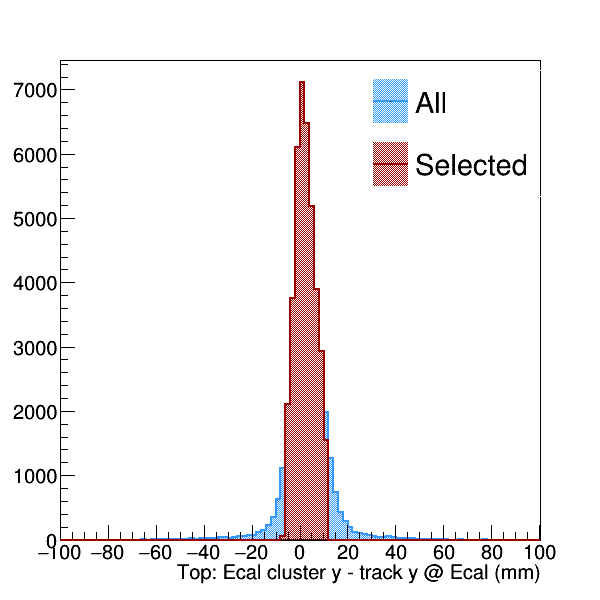
\includegraphics[width=0.85\textwidth]{images/20160502_pass4_cluster_track_delta_y_top.png}
    \end{subfigure}
    \begin{subfigure}{.5\textwidth}
        \centering
        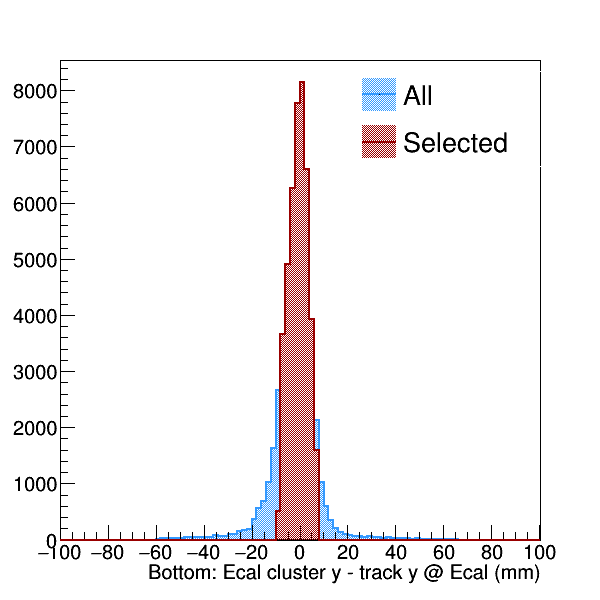
\includegraphics[width=0.85\textwidth]{images/20160502_pass4_cluster_track_delta_y_bottom.png}
    \end{subfigure}
    \caption{Histogram}
    \label{fig:track_cluster_delta_y}
\end{figure}
\begin{table}[t]
    \begin{center}
        \begin{tabular}{r|cc}
            \hline
                    & Cluster x - track x at Ecal (mm) &  Cluster y - track y at Ecal (mm)  \\
            \hline
            Top     & $\ge -6.10$ and $\le 12.93$ & $\ge -6.08$ and $\le 11.49$ \\ 
            Bottom  & $\ge -8.02$ and $\le 10.84$ & $\ge -8.31$ and $\le 7.40$  \\ 
            \hline
        \end{tabular}
    \end{center}
    \caption{Boundaries used to denote the 3$\sigma$ window used to establish if 
             an Ecal cluster and SVT track are matched to each other.  Due to 
             global misalignments, different windows are needed for top and 
             bottom tracks and clusters.}
    \label{tab:track_cluster_cuts}
\end{table}
If multiple tracks were found to match to a single cluster, the track 
with the minimum radial distance to the cluster was chosen.  

\subsection{Final Trident Sample}

The event selection criteria that have been applied thus far only select 
events that have QED trident or $A'$ like signatures i.e. two coincident clusters that
passed the trigger cuts and have $e^+e^-$ tracks associated with them.  However, 
there remains several $e^+e^-$ accidentals that need to be removed from the final 
event sample.  This is best accomplished by subjecting the tracks associated 
with the clusters to the following additional criteria:
\begin{itemize}
    \item For simplicity, events that have multiple positron tracks are not 
          considered.
    \item In order to cut down on the number of misconstructed tracks that may
          have been mismatched to a cluster, both tracks are subjected to 
          $\chi^2$ probability cut of 95\%.
    \item Some of the electrons in the cluster pair may actually be a multiple
          Coulomb scattered beam electron of energy 1.056 GeV 
          instead of one associated with a true $e^+e^-$ 
          pair.  To remove these events from the final event sample, the 
          momentum of electron tracks are required to be less than 0.85 GeV.
    \item The $e^+e^-$ tracks associated with the clusters are vertexed with 
          their position along the beamline, $v_z$, constrained to the target. 
          For true $e^+e^-$ pairs, the vertex position in x and y ($v_x$ and $v_y$) should be
          well constrained to an ellipse with dimensionality close to the beam 
          spot.  With this in mind, the fitted vertex $\chi^2$ is first required 
          to be less than 10.  The positions along x and y are then required 
          to lie within an ellipse 
          defined as
          \[
                v_x^2/0.04 + v_y^2/0.0025  = 1.
          \]
          The elliptical selection is shown graphically on Fig. \ref{fig:vertex_xy}.
\end{itemize}
%%%%%%%%%%%%%%
%   Figure   %
%%%%%%%%%%%%%%
\begin{figure}[t]
    \centering
    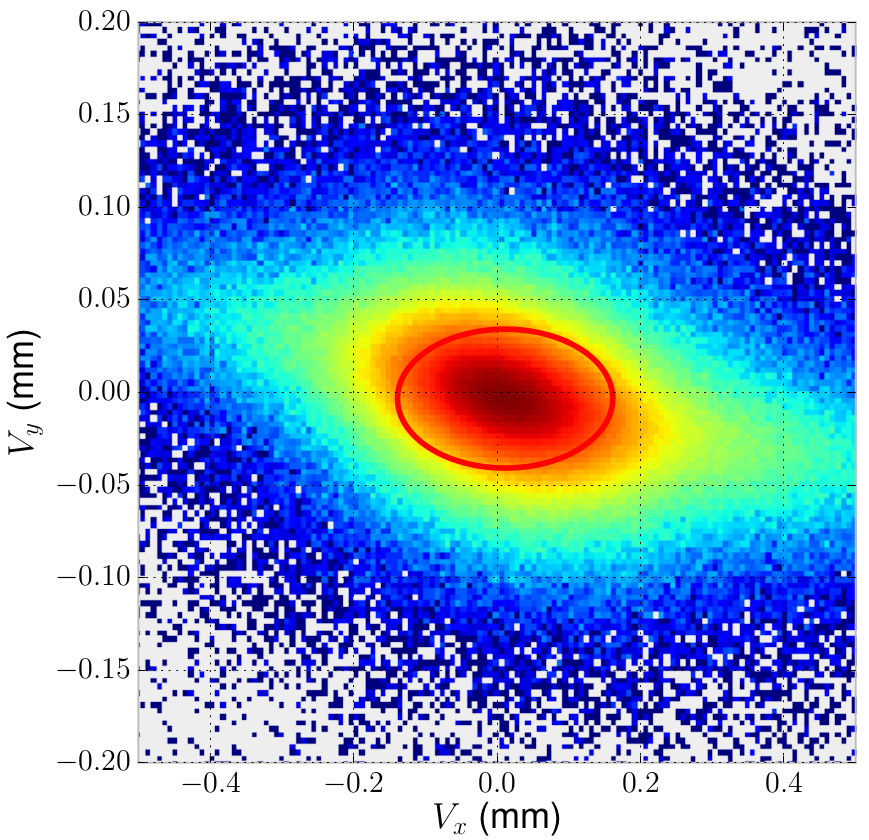
\includegraphics[width=.7\textwidth]{images/20160503_vertex_xy.png}
    \caption{Vertex position at the target.}
    \label{fig:vertex_xy}
\end{figure}  
%%%%%%%%%%%%%%
%   Figure   %
%%%%%%%%%%%%%%

\subsection{Radiative Selection}

As discussed in Chapter 2, the kinematic similarities between heavy photons and
radiative processes can be used to analyze both the rate of $A'$ signal production
and the sensitivity of the experiment to $A'$ signals.  It is then crucial to
maximize the fraction of radiative events in the final event sample.  The final
event sample is expected to be dominated by the Bethe-Heitler process.  However,
the kinematic difference between the radiative and Bethe-Heitler processes can 
be exploited to reduce the number of Bethe-Heitler events.  Specifically, the 
$e^+e^-$ pair produced in a radiative process will be highly boosted, while 
only one of the electrons in the Bethe-Heitler process will be boosted 
while the other will be much softer.  With this in mind, the sum of the momentum
of the electron and positron, ``p-sum'', allows the discrimination between the two processes.
Specifically, radiative events are expected to have a ``p-sum'' peaked 
closed to the beam energy, while the distribution of Bethe-Heitlers will be peaked a 
low p-sum.

Figure \ref{fig:p_sum} shows the distribution of the sum of the momentum of the $e^+e^-$ tracks composing a 
%%%%%%%%%%%%%%
%   Figure   %
%%%%%%%%%%%%%%
\begin{figure}[t]
    \centering
    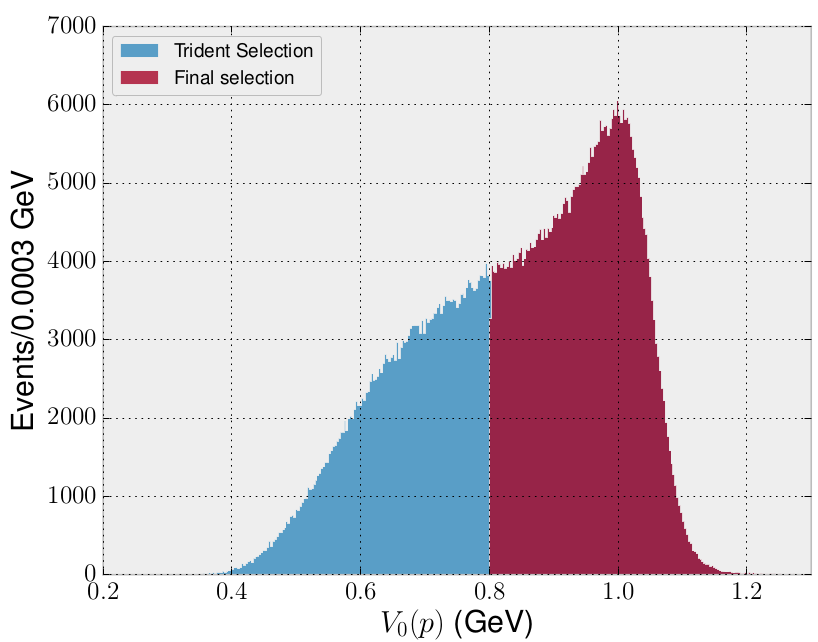
\includegraphics[width=.7\textwidth]{images/20160504_psum.png}
    \caption{Distribution of the sum of $e^+e^-$ momentum.  The distribution in 
             red graphically indicates the selection used to maximize the fraction
             of  radiative events in the final event sample.}
    \label{fig:p_sum}
\end{figure}  
%%%%%%%%%%%%%%
%   Figure   %
%%%%%%%%%%%%%%
pair. Using pure radiative and full trident Monte Carlo, requiring a pair to have a 
p-sum cut greater than 0.8 GeV was found to maximize the radiative fraction.
The cut is shown graphically on Fig. \ref{fig:p_sum}.  The invariant mass
distribution before (blue) and after (red) the p-sum cut was applied is also shown
on Fig. \ref{fig:mass_selection}.

\begin{figure}[t]
    \centering
    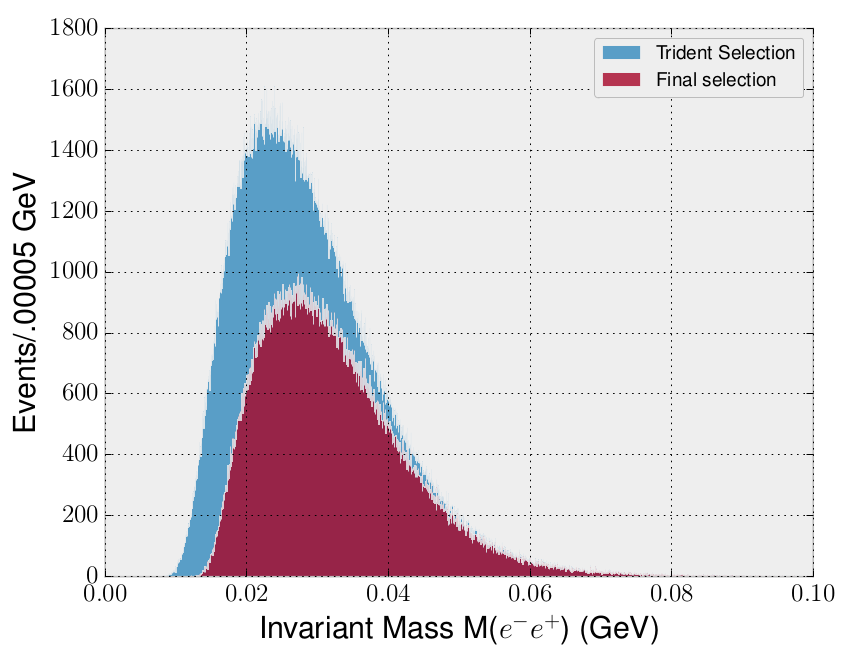
\includegraphics[width=1.0\textwidth]{images/20160504_invariant_mass_selection.png}
    \caption{The Heavy Photon Search $e^+e^-$ invariant mass distribution before (blue) 
             and after (red) a cut on the sum of the $e^+e^-$ momentum.  The cut 
             maximizes the number of radiative trident events in the final event sample.
             The mass distribution in red 
             will serve as the starting point for the resonance search.}
    \label{fig:mass_selection}
\end{figure}

%\subsection{Event Selection Efficiencies}


%%%%%%%%%%%%%%%%%%%%%%%%
%   Resonance Search   %
%%%%%%%%%%%%%%%%%%%%%%%%

\chapter{Resonance Search and Results} \label{chap:resonance}

The following chapter will discuss the details and results of a resonance 
search for an $A'$ in the mass range between 20 MeV/$c^2$ to 60 MeV/$c^2$.
This includes a discussion of the procedure used to determine if a significant
resonance was observed at a given $A'$ mass hypothesis and the statistical
formalism used to set an upper limit on both the signal and $A'$ coupling
strength.

This analysis makes use of
the unblinded portion of the 2015 HPS engineering run data which amounts to 
a luminosity of 74 nb$^{-1}$ (.4671 mC of charge) or 1/10 of a PAC day.  
A blind search for a resonance using the procedure outlined in this chapter 
and making use of the full 2015 engineering run 
dataset (1165.71 nb$^{-1}$, 7.2875 mC) is expected to be completed in the 
Summer of 2016.

\section{Searching for a Resonance}

If a heavy photon does indeed exist and has a mass that is within the acceptance
of the HPS detector, it will appear as a resonance above the copious QED trident
invariant mass distribution.  Such a signal is expected to be Gaussian in 
nature, with a mean equal to the mass of the $A'$, $m_{A'}$, and with a mass
dependent width, $\sigma_{m_{A'}}$, given by the mass resolution 
parameterization define in Section \ref{sec:mass_res}. With this in mind, the 
invariant mass distribution measured by HPS (see Chapter 
\ref{ch:event_selection} and Fig. \ref{fig:mass_selection}) will serve as the
starting point for this analyses. 
%In total, the invariant
%distribution contains 437,766 events binned into a histogram ranging between 
%0 and .1 GeV and bin sizes of 0.00005 GeV.
%\begin{figure}[t]
%    \centering
%    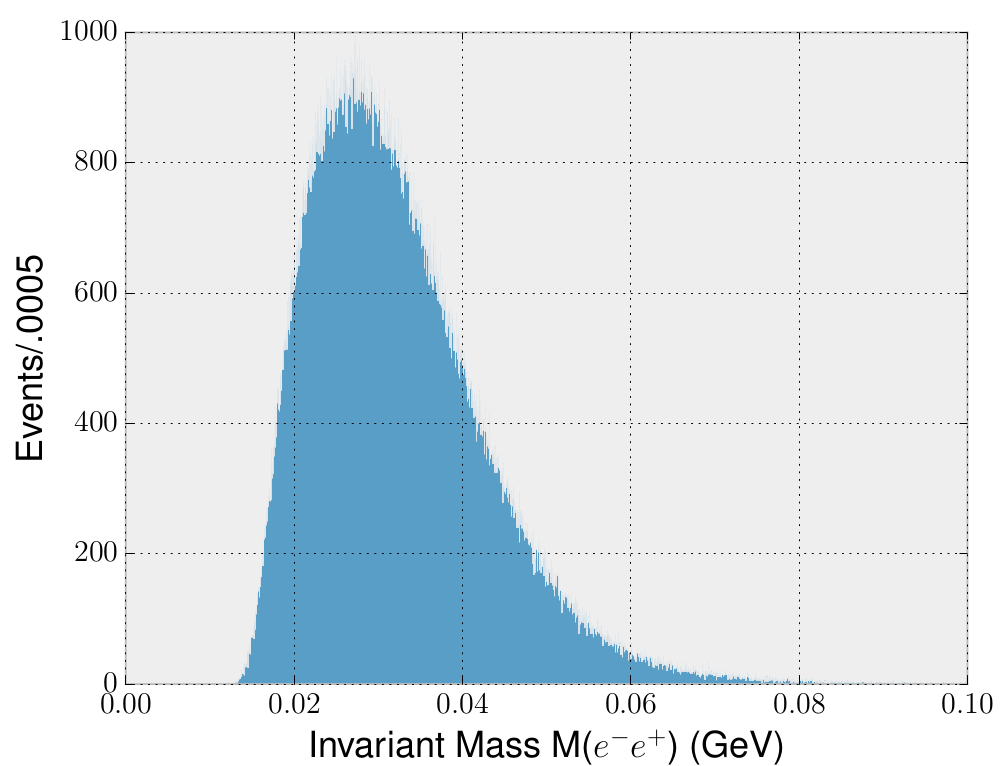
\includegraphics[width=1.0\textwidth]{images/invariant_mass_final.png}
%    \caption{The Heavy Photon Search $e^+e^-$ invariant mass distribution after
%             the final event selection has been applied.  The mass distribution
%             will serve as the starting point for the resonance search.}
%    \label{fig:mass_distribution}
%\end{figure}

\subsection{Maximum Likelihood Fit}

Since the mass of the $A'$ is unknown a priori, the 
$e^+e^-$ invariant mass spectrum needs to be scanned for any significant peaks.
Customarily, a search for a resonance is performed within a
window constructed around the mass hypothesis of interest.  Within the window,
the distribution of $A'$ signal events is modeled using the probability 
distribution function
\begin{equation}
    \begin{split}
    P(m_{e^+e^-}) 
        = 
        \mu \cdot \phi(m_{e^+e^-} | m_{A'}, \sigma_{m_{A'}}) + B\cdot p(m_{e^+e^-} | t_j)
    \end{split}
\end{equation}
where $m_{e^+e^-}$ is the $e^+e^-$ invariant mass, $\mu$ is the signal yield,
$B$ is the number of background events within the window, 
$\phi(m_{e^+e^-} | m_{A'})$ is a Gaussian probability distribution describing
the signal and $p(m_{e^+e^-} | t_j)$ is a Chebyshev polynomial of the first kind
with coefficients $t_j$ that is used to describe the background shape.
Estimating the 
signal yield as well the background normalization and shape within a window, can be
done by the method of maximum likelihood.  The theoretical formalism
used to do this will be outlined here but a detailed discussion can be found in
\cite{Cowan:2010js}.

Assume the events within the window are binned as $\mathbf{n} = (n_{1}, ... n_{i})$.
Furthermore, assume the center of the $i$th bin is given by $b_i$ and has a width
equal to $\epsilon$. 
The expected number of events of the $i$th bin is given by 
\begin{equation}
    E[n_i] = S_{i} + B_{i}
\end{equation}
where 
\begin{equation}
    S_{i} = \mu \int_{b_i - \epsilon/2}^{b_i + \epsilon/2} \phi(m_{e^+e^-} | m_{A'}, \sigma_{m_{A'}}) d (m_{e^+e^-})
\end{equation} 
\begin{equation}
    B_{i} = B_{total} \int_{b_i - \epsilon/2}^{b_i + \epsilon/2} p(m_{e^+e^-} | t_{j}) d (m_{e^+e^-}).
\end{equation}
Denoting the parameters that are not of immediate interest, i.e. the nuissance
parameters, by $\theta = (B_{total},  t_{j})$, an estimation
of $\mu$ and $\theta$ can be obtained by finding the parameters $\hat{\mu}$ and
$\hat{\theta}$ that maximize the Poisson likelihood function, $\mathcal{L}$
\begin{equation}
\mathcal{L}(\mu, \theta) = \prod_{k=1}^{n_{\text{bins}}} \frac{(S_{k} + B_{k})^{n_k}}{n_{k}!} e^{-(S_{k} + B_{k})}
\end{equation}
where the sum is over all bins within the window, $n_{\text{bins}}$.
In the case where the invariant mass is scanned for a resonance, the Poisson 
likelihood function is maximized within the window constructed around each
$A'$ mass hypothesis. This yields estimators for the signal yield and nuissance
parameters at each $A'$ mass hypothesis which are used to determine if a significant 
resonance was found.

\subsection{Likelihood Ratio} \label{sub:likelihood_ratio}

When searching for a resonance above a background distribution, it is 
necessary to discriminate between two scenarios:
\begin{itemize}
    \item The background only or null hypothesis, $H_{0}: \mu = 0$.
    \item The signal+background hypothesis or alternative, $H_{1}: \mu > 0$.
\end{itemize}
Establishing whether the signal+background model is significantly different 
from the background only model is typically done using the profile likelihood
ratio
\begin{equation}
    \lambda(\mu) = \frac{\mathcal{L}(\mu, \hat{\hat{\theta}})}{\mathcal{L}(\hat{\mu}, \hat{\theta})}
    \label{eqn:likelihood_ratio}
\end{equation}
where $\hat{\hat{\theta}}$ is the conditional estimator for the nuissance parameters 
obtained by maximizing the Poisson likelihood assuming that the null or 
background only hypothesis is true i.e. $\mu = 0$. The unconditional estimators $\hat{\mu}$ 
and $\hat{\theta}$ are obtained by maximizing the Poisson likelihood without
any constraints on $\mu$.
As can be seen from \ref{eqn:likelihood_ratio}, 
if the estimator of the signal yield, $\hat{\mu}$, is compatible (incompatible)
with the hypothesized $\mu$, the likelihood ratio will tend to 1 (0).

A more convenient test statistic is the log likelihood ratio defined as
\begin{equation}
    q_0 = \begin{cases}
            -2 \ln \frac{\mathcal{L}(0, \hat{\hat{\theta}})}{\mathcal{L}(\hat{\mu}, \hat{\theta})} 
            & \hat{\mu} > 0 \\
             0  & \hat{\mu} < 0.
        \end{cases}
\end{equation}
In the large sample limit, the test statistic
$q_0$ can be shown to follow a $1/2\chi^2$ distribution defined in \cite{Cowan:2010js} as 
\begin{equation}
    f(q_{0}|0) = \frac{1}{2} \left(\delta(q_{0}) + \frac{1}{\sqrt{2\pi}}\frac{1}{\sqrt{q_{0}}}e^{-q_0/2} \right)
    \label{eqn:half_chi}
\end{equation}
where the first term on the right side of the equation is a delta function at 0
and the second term is a $\chi^2$ distribution with one degree of freedom. 
%Equation \ref{eqn:half_chi} is simple the mixture 
%is asymptotically $1/2\chi^2$ \footnote{The 1/2 comes from the fact that only
%signal yields greater than 0 are being considered. See \cite{Cowan:2010js} for a 
%more detailed explanation.} distributed with degrees of freedom equal to the
%difference in parameters between the two models being tested.  In our current case, 
%the number of degrees of freedom is one, since the signal yield is the only 
%parameter that does not appear in
%the background only model.

Quantifying how extreme the observation is can be done by calculating a $p$-value as
\begin{equation}
    p = \int_{q_{0,obs}}^{\infty} f(q_{0} | 0) dq_{0}.
\end{equation} 
This is shown graphically on Fig. \ref{fig:p_value}.  Typically, the observed 
p-value is
\begin{figure}[t]
    \centering
    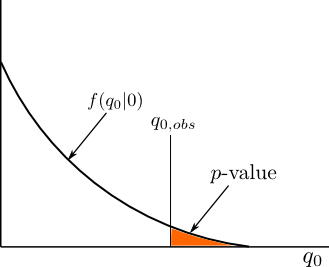
\includegraphics[width=.5\textwidth]{images/p_value.png}
    \caption{Graphical representation of a p-value.}
    \label{fig:p_value}
\end{figure}
compared against a significance level $\alpha$.  The significance level denotes
the probability of incorrectly rejecting the null hypothesis in favor of the 
alternative (type-I error).  In other words, it denotes the probability of there
being a statistical fluctuation in the background large enough to mimic a signal.  
If a $p$-value is 
found to be less than $\alpha$, the measurement is claimed to be significant. 
Typically, in particle 
physics, an $\alpha$ on the order of $3 \times 10^{-7}$ (5$\sigma$) is required
to claim discovery of new phenomena.  This means that there is a 1 in 
about 3.5 million chance that the observation is due to a fluctuation in the background.

\subsection{The Look-Elsewhere Effect}

As discussed previously in Section \ref{sub:likelihood_ratio}, a result is 
determined significant if the $p$-value is smaller than some pre-determined
threshold, $\alpha$.  However, 
when performing multiple test, as is the case when scanning a mass distribution
for a resonance, an observation with a $p$-value that is as extreme as $\alpha$
is bound to occur at a rate of $n\times\alpha$ where $n$ is the number of measurements.
This phenomena is known as the ``Look-Elsewhere Effect'' (LEE)
and needs to be taken into account through a correction to the ``local'' $p$-value
observed at each mass hypothesis.

Assuming that only a single heavy photon can be observed within the HPS invariant
mass distribution, the correction can be estimated using a large number
of pseudo-data sets and generating the distribution 
$f(q_{0, max} | 0)$ composed of the largest $q_{0}$ (i.e. smallest $p$-value)
from each of the invariant mass scans.
%The distribution $f(q_{0, max} | 0)$ can
%be derived by running a large number of pseudo-experiments and then calculating
%the $p$-value as was explained previously.
However, generating a distribution of $f(q_{0, max} | 0)$ that would allow 
an estimation of a ``global''  
$p$-value (i.e. local $p$-value after correction) down to the level of 5$\sigma$ with any accuracy would 
require running $> 10^{6}$ pseudo experiments.  Generating so many pseudo-data 
sets is often not feasible within a reasonable amount of time. 

Instead, the smallest
$p$-values obtained from a series of resonance searches on 10,000 pseudo
data sets were
ranked and the corresponding quantile was calculated \cite{Gross:2010qma}.  
A mapping from a local 
$p$-value to a global $p$-value is then created.  The mapping created 
for this analysis is shown on Figure \ref{fig:global_p_value}.
\begin{figure}[t]
    \centering
    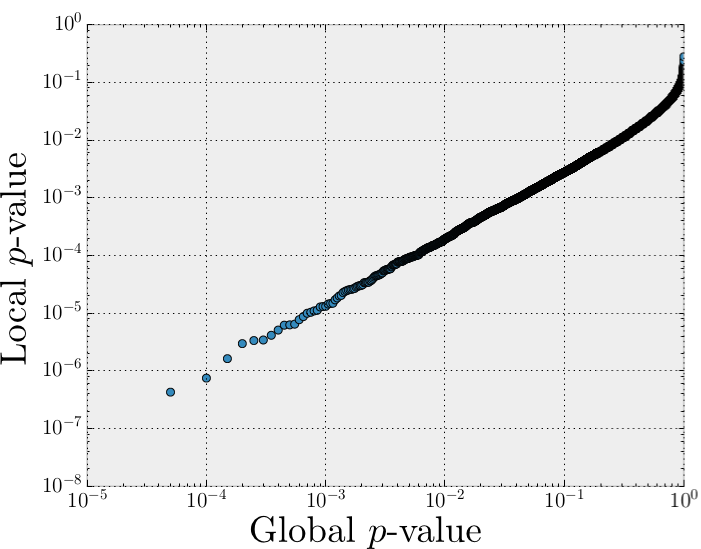
\includegraphics[width=\textwidth]{images/global_p_value_map.png}
    \caption{Mapping between local and global p-values.}
    \label{fig:global_p_value}
\end{figure}
As can be seen from the figure, a 
local $p$-value equal to 0.05 corresponds to a global $p$-value of $\sim$ 0.5.

\section{Fit Parameters}

Prior to performing the resonance search on real data, several fit parameters 
were optimized using pseudo data sets based on Monte Carlo.  These included the size of the fit 
window, the binning of the invariant mass distribution and the order of 
the polynomial used to describe the background.  All parameters were chosen 
such that signal yield pull
\begin{equation}
    \text{pull} = \frac{\mu_{\text{fit}} - \mu_{\text{inserted}}}{\mu_{\text{fit error}}}
\end{equation}
was minimized for all fits performed across an invariant mass spectrum.

\subsection{Pseudo Data Sets}

\begin{figure}[ht]
    \centering
    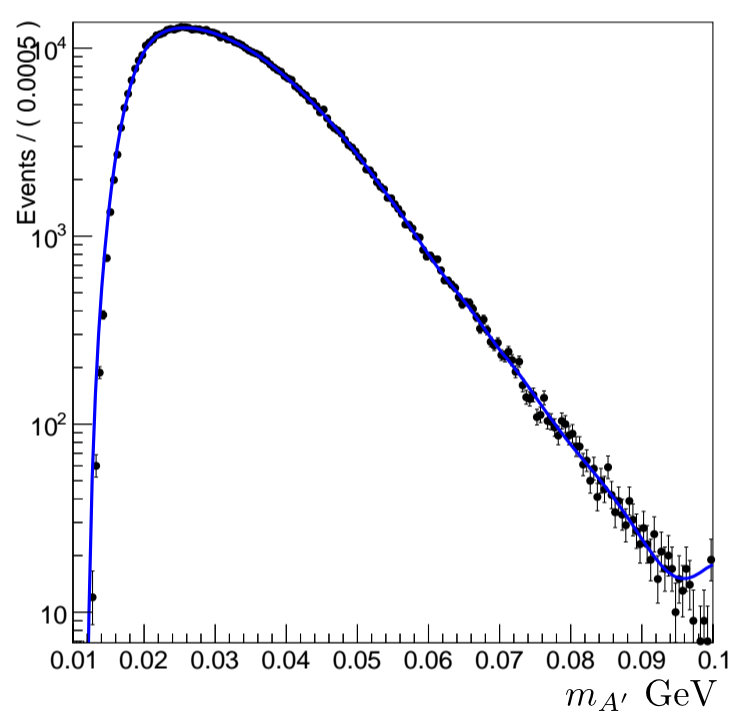
\includegraphics[width=0.7\textwidth]{images/smooth_pdf.png}
    \caption{Probability density function obtained by applying a smoothing algorithm 
             to the Heavy Photon Search Monte Carlo invariant mass distribution.}
    \label{fig:smooth_pdf}
\end{figure}

Pseudo data sets are needed to understand fitting systematics and to optimize
the fit function, window size and mass binning.  In order to obtain an invariant
mass probability
density function (PDF) that describes the data, smoothing algorithm 353 QH 
\cite{Friedman:1974vj} was
%What smoothing algorithm was used? Why? Was a K-S test used to make sure the
% resulting PDF matched the data set?
applied to the unit normalized final invariant mass MC distribution.  The resulting
PDF after smoothing (blue line) overlaid on top of the MC distribution it was generated 
from is shown on Fig. \ref{fig:smooth_pdf}.  

Pseudo data sets were then generated
by sampling the PDF between 0 and 100 MeV with the total number of
%events, 437,766,
events, 437,766, chosen to match the number observed in data.  The resulting
pseudo data is binned to match the data distributions with the expectation
value of each bin Poisson distributed.

%% What kind of sampling algorithm was used? 

\subsection{Mass Binning}

Ideally, an unbinned maximum likelihood fit would be used to estimate the fit 
parameters describe previously.  However, due to the large number of statistics, 
this wouldn't be possible to do in a reasonable amount of time.  Instead, 
a binned likelihood fit is performed with the bin size set such that the 
pulls are minimized.

In order to understand the effect of the bin size on the fitting systematics, 
pseudo data sets were binned using bin sizes of 0.2 MeV, 0.1 MeV and 0.05 MeV.
A resonance search was performed on each of the pseudo data sets and pull 
distributions were generated at 
%mean pull at
each mass hypothesis.
%was calculate.
Using this procedure, it was found that using
a bin size of 0.05 MeV minimizes the pulls, hence, it was used in the final
analysis.

\subsection{Fit Window and Polynomial Order}

The pseudo data sets were also used to understand what size fit window and what 
order polynomial minimizes the signal yield pulls. Performing a resonance search on 
each of the pseudo data sets using windows of size $n \times \sigma_{m_{A'}(m_{e^+e^-})}$
where $n$ is a scale factor, it was found that $n = 15$ minimizes the pulls 
across the whole range. Furthermore, it was found that the maximum window
size that could be used is 20 MeV after which the pulls would become worse. 
A similar procedure was used to determine the polynomial used to model the background.
It was found that a 7th order polynomial minimizes the pulls. 

\section{Results}

The resulting local $p$-values from a resonance search conducted in the range 
between 20 MeV and 60 MeV are shown on Fig. \ref{fig:local_p_values}. 
The most significant signal
was found at a mass of 27.525 MeV and has a local p-value of $4 \times 10^{-3}$.
The resulting signal plus background fit (blue) along with the signal component 
(red) and background component (green) is shown on Figure \ref{fig:fit_27}.
After correcting for the LEE, the corresponding global p-value is 
$\sim 10\%$.
\begin{figure}[t]
    \centering
    \includegraphics[width=\textwidth]{images/final_p_values.png}
    \caption{Resulting $p$-values from a resonance search for an $A'$ across the
    invariant mass spectrum.}
    \label{fig:local_p_values}
\end{figure}

\begin{figure}[ht]
    \centering
    \includegraphics[width=.6\textwidth]{images/fit27.png}
    \caption{Resulting signal plus background fit (blue) assuming an $A'$ mass hypothesis
             of 27.525 MeV.  The signal component is shown in red while the 
         background component is shown in green.}
        
    \label{fig:local_p_values}
\end{figure}

\section{Setting Upper Limits on the Signal Yield}

Since no significant resonances were found, a 90\% confidence upper limit on the number
of signal events at each mass hypothesis was set.  For the purpose of setting
an upper limit, the likelihood ratio is inverted.  The statistic used
to set an upper limit is then
\begin{equation}
    q_{\mu} = \begin{cases}
        -2 \ln \frac{\mathcal{L}(\mu, \hat{\hat{\theta}})}{\mathcal{L}(0, \hat{\hat{\theta}})} 
            & \hat{\mu} < 0 \\
        -2 \ln \frac{\mathcal{L}(\mu, \hat{\hat{\theta}})}{\mathcal{L}(\hat{\mu}, \hat{\theta})} 
            & 0 \leq \hat{\mu} \leq \mu \\
             0  & \hat{\mu} > \mu
        \end{cases}
\end{equation}
with the corresponding $p$-value being given by
\begin{equation}
    p = \int_{q_{\mu,obs}}^{\infty} f(q_{\mu} | \mu) dq_{\mu}
\end{equation}
where $f(q_{\mu}|\mu)$ is the probability distribution of $q_{\mu}$ given the
hypothesized value of $\mu$. 
In order to find the upper limit, $\mu_{\text{up}}$, the test above is carried out over a range of
signal yields until a $p$-value of 0.1 (90\% confidence) is found.  The signal
yield value that corresponds to a $p$-value of 0.1 is $\mu_{\text{up}}$
and is often referred to as the unconstrained limit. 
%The value of
%$\mu_{\text{up}}$ found in this way
%is often referred to as the unconstrained limit.
The resulting 
unconstrained upper limits are shown in blue on Fig. \ref{fig:upper_limit}. 
\begin{figure}[t]
    \centering
    \includegraphics[width=\textwidth]{images/upper_limits.png}
    \caption{Upper limits on the signal yield at each mass hypothesis.}
    \label{fig:upper_limit}
\end{figure}

As shown in green on Fig. \ref{fig:upper_limit}, it is often the case that the
estimator for the signal yield, at a given mass hypothesis is zero or
even negative.  In such cases, the probability distribution function of the
test statistic $q_{\mu}$ assuming $\mu_{\text{up}}$ will nearly coincide with 
the distribution of $q_{\mu}$ assuming $\mu = 0$, i.e. the background only 
hypothesis.  As a result, there is a lack of 
sensitivity to a signal measurement at those mass hypothesis.

In such cases, a 50\% power-constrained upper limit on the signal is set
\cite{Cowan:2011an}.
At each mass hypothesis, a distribution of signal upper limits is generated from
background only pseudo-data sets and the median (50\% quantile) upper limit
is calculated, $\mu_{\mbox{median}}$. The upper limit in that region is then set to 
the larger of either the unconstrained limit or the median limit
\begin{equation}
    \mu_{pc} = \mbox{max}(\mu_{\text{up}}, \mu_{\text{median}}).
\end{equation}
The power constrained limits are shown in red on Fig. \ref{fig:upper_limit}.

\section{Setting a limit on $\epsilon$}

As discussed in chapter 2, the kinematic similarities between heavy photons and 
radiatives allows their cross sections to be related within a mass window, 
$\delta m$, near $m_{A'}$ as 
\begin{equation}
    \frac{d\sigma(e^-Z \rightarrow e^-A'Z(A' \rightarrow e^+e^-))}{
    d\sigma(e^-Z \rightarrow e^-\gamma^*Z(\gamma^* \rightarrow e^+e^-))} = 
    \left( \frac{3 \pi \epsilon^2}{2 N_{eff} \alpha} \right)
        \left( \frac{m_{A'}}{\delta m_{A'}} \right)
    \label{eqn:ap_rad_xsec}
\end{equation}
where $N_{eff}$ is the number of available decay channels available.  For the 
$A'$ masses considered in this analysis, $N_{eff} = 1$. Using equation 
\ref{eqn:ap_rad_xsec}, the upper limit on the signal, $S_{\text{up}}$, can be related to an
upper limit on the $A'$ coupling strength as 
\begin{equation}
    \epsilon^2 = \left (\frac{S_{\text{up}}/m_{A'}}{
                f\Delta B/\Delta m} \right) 
                \left(\frac{2 N_{eff} \alpha}{3 \pi} \right)
    \label{eqn:eps}
\end{equation}
where $\Delta B/\Delta m$ is the number of 
background events per MeV and $f$ is the ratio of the pure radiative cross-section to the full trident 
cross section.  The ratio is calculated using MC and is shown on Figure \ref{fig:rad_frac} as 
a function of mass.
In order to calculate the number of background 
events per MeV, a 1 MeV window is constructed around the $A'$ mass hypothesis
and the number of background events in that window are counted.  The resulting 
number of background events per MeV at each mass hypothesis are shown on Fig. 
\ref{fig:background_mev}.  

The limits on the coupling strength derived using equation \ref{eqn:eps}
are shown on Fig. \ref{fig:epsilon_upper_limit}. Using the full data set
the reach is expected to increase by a factor of ~4 down to $\epsilon^2 \sim 10^{-6}$.
\begin{figure}[ht]
    \centering
    \includegraphics[width=.8\textwidth]{images/rad_frac.png}
    \caption{The ratio of the pure radiative cross-section to the full trident 
             cross section as a function of mass.}
    \label{fig:rad_frac}
\end{figure}
\begin{figure}[hb]
    \centering
    \includegraphics[width=\textwidth]{images/bkg_mev.png}
    \caption{The number of background events in a 1 MeV window around each $A'$ mass hypothesis.}
    \label{fig:background_mev}
\end{figure}
\begin{figure}[ht]
    \centering
    \includegraphics[width=\textwidth]{images/final_coupling_upper_limits.png}
    \caption{Upper limits on the coupling strength.}
    \label{fig:epsilon_upper_limit}
\end{figure}







%%%%%%%%%%%%%%%%%%%%
%   Bibliography   %
%%%%%%%%%%%%%%%%%%%%
\bibliographystyle{hunsrt}
\bibliography{chapters/bibliography}

\end{document}
